%Dokumenteinstellungen und Anpassungen
%Dokumentenklasse "scrbook" - Erweitert um den Verweis auf die Verzeichnisse und Texteigenschaften
\documentclass[chapterprefix=true, 12pt, a4paper, oneside, parskip=half, listof=totoc, bibliography=totoc, numbers=noendperiod]{scrbook}


%Anpassung der Seitenränder (Standard bottom ca. 52mm anbzüglich von ca. 4mm für die nach oben rechts gewanderte Seitenzahl)
\usepackage[bottom=48mm,left=25mm,right=25mm]{geometry}

%Tweaks für scrbook
\usepackage{scrhack}

%Blindtext
\usepackage{blindtext}

%Erlaubt unteranderem Umbrücke captions
\usepackage{caption}

%Stichwortverzeichnis
\usepackage{imakeidx}

%Kompakte Listen
\usepackage{paralist}

%Zitate besser formatieren und darstellen
\usepackage{epigraph}

%Glossar, Stichworverzeichnis (Akronyme werden als eigene Liste aufgeführt)
\usepackage[toc, acronym]{glossaries} 

%Anpassung von Kopf- und Fußzeile
%beinflusst die erste Seite des Kapitels
\usepackage[automark,headsepline]{scrlayer-scrpage}
\automark{chapter}
\ihead{\leftmark}
\chead{}
\ohead{\thepage}
\ifoot*{}
\cfoot[\thepage]{}
\cfoot*{}
\ofoot*{\thepage}
\ofoot{}
\pagestyle{scrheadings}


%Auskommentieren für die Verkleinerung des vertikalen Abstandes eines neuen Kapitels
%\renewcommand*{\chapterheadstartvskip}{\vspace*{.25\baselineskip}}

%Zeilenabstand 1,5
\usepackage[onehalfspacing]{setspace}

%Verbesserte Darstellung der Buchstaben zueinander
\usepackage[stretch=10]{microtype}

%Deutsche Bezeichnungen für angezeigte Namen (z.B. Innhaltsverzeichnis etc.)
\usepackage[ngerman]{babel}

%Unterstützung von Umlauten und anderen Sonderzeichen (UTF-8)
\usepackage{lmodern}
\usepackage[utf8]{luainputenc}
\usepackage[T1]{fontenc}

%Einfachere Zitate
\usepackage{epigraph}

%Unterstützung der H positionierung (keine automatische Verschiebung eingefügter Elemente)
\usepackage{float} 

%Erlaubt Umbrüche innerhalb von Tabellen
\usepackage{tabularx}

%Erlaubt Seitenumbrüche innerhalb von Tabellen
\usepackage{longtable}

%Erlaubt die Darstellung von Sourcecode mit Highlighting
\usepackage{listings}

%Definierung eigener Farben bei nutzung eines selbst vergebene Namens
\usepackage[table,xcdraw]{xcolor}

%Vektorgrafiken
\usepackage{tikz}

%verschiedene Schriftfarben
\usepackage{xcolor}
\definecolor{htw_green}{RGB}{112, 173, 71}

%Grafiken (wie jpg, png, etc.)
\usepackage{graphicx}
\usepackage{adjustbox}

%Grafiken von Text umlaufen lassen
\usepackage{wrapfig}

%Ermöglicht Verknüpfungen innerhalb des Dokumentes (e.g. for PDF), Links werden durch "hidelink" nicht explizit hervorgehoben
\usepackage[hidelinks,german]{hyperref}

%Einbindung und Verwaltung von Literaturverzeichnissen
\usepackage{csquotes} %wird von biber benötigt
\usepackage[style=alphabetic, backend=biber, bibencoding=ascii]{biblatex}
\addbibresource{references/references.bib}
%Anpassung der Überschriften
\addtokomafont{disposition}{\rmfamily}

%Zusätzliche Farben
\definecolor{darkgreen}{RGB}{0,100,0}

%Umbenennungen
\renewcommand{\lstlistlistingname}{Quelltextverzeichnis}

%Pluszeichen in der Referenc beim zitieren ausblenden
\renewcommand*{\labelalphaothers}{}

%Anpassugen zur Quelltextdarstellung, kann bei Bedarf überschrieben werden (z.B. wenn unterschiedliche Sprachen zum Einsatz kommen)
\renewcommand{\lstlistingname}{Codeauszug}
\lstset{
	numbers=left,
	columns=fullflexible,
	aboveskip=5pt,
	belowskip=10pt,
	basicstyle=\small\ttfamily,
	backgroundcolor=\color{black!5},
	commentstyle=\color{darkgreen},
	keywordstyle=\color{blue},
	stringstyle=\color{gray},
	showspaces=false,
	showstringspaces=false,
	showtabs=false,
	xleftmargin=16pt,
	xrightmargin=0pt,
	framesep=5pt,
	framerule=3pt,
	frame=leftline,
	rulecolor=\color{green},
	tabsize=2,
	breaklines=true,
	breakatwhitespace=true,
	prebreak={\mbox{$\hookleftarrow$}}
}

\lstdefinelanguage{CSS}{
	keywords={color,background-image:,margin,padding,font,weight,display,position,top,left,right,bottom,list,style,border,size,white,space,min,width, transition:, transform:, transition-property, transition-duration, transition-timing-function},	
	sensitive=true,
	morecomment=[l]{//},
	morecomment=[s]{/*}{*/},
	morestring=[b]',
	morestring=[b]",
	alsoletter={:},
	alsodigit={-}
}

% JavaScript
\lstdefinelanguage{JavaScript}{
	morekeywords={typeof, new, true, false, catch, function, return, null, catch, switch, var, if, in, while, do, else, case, break},
	morecomment=[s]{/*}{*/},
	morecomment=[l]//,
	morestring=[b]",
	morestring=[b]'
}

\lstdefinelanguage{HTML5}{
	language=html,
	sensitive=true,	
	alsoletter={<>=-},	
	morecomment=[s]{<!-}{-->},
	tag=[s],
	otherkeywords={
		% General
		>,
		% Standard tags
		<!DOCTYPE,
		</html, <html, <head, <title, </title, <style, </style, <link, </head, <meta, />,
		% body
		</body, <body,
		% Divs
		</div, <div, </div>, 
		% Paragraphs
		</p, <p, </p>,
		% scripts
		</script, <script,
		% More tags...
		<canvas, /canvas>, <svg, <rect, <animateTransform, </rect>, </svg>, <video, <source, <iframe, </iframe>, </video>, <image, </image>, <header, </header, <article, </article
	},
	ndkeywords={
		% General
		=,
		% HTML attributes
		charset=, src=, id=, width=, height=, style=, type=, rel=, href=,
		% SVG attributes
		fill=, attributeName=, begin=, dur=, from=, to=, poster=, controls=, x=, y=, repeatCount=, xlink:href=,
		% properties
		margin:, padding:, background-image:, border:, top:, left:, position:, width:, height:, margin-top:, margin-bottom:, font-size:, line-height:,
		% CSS3 properties
		transform:, -moz-transform:, -webkit-transform:,
		animation:, -webkit-animation:,
		transition:,  transition-duration:, transition-property:, transition-timing-function:,
	}
}

\lstdefinestyle{htmlcssjs} {%
	% General design
	%  backgroundcolor=\color{editorGray},
	basicstyle={\footnotesize\ttfamily},   
	frame=b,
	% line-numbers
	xleftmargin={0.75cm},
	numbers=left,
	stepnumber=1,
	firstnumber=1,
	numberfirstline=true,	
	% Code design
	identifierstyle=\color{black},
	keywordstyle=\color{blue}\bfseries,
	ndkeywordstyle=\color{editorGreen}\bfseries,
	stringstyle=\color{editorOcher}\ttfamily,
	commentstyle=\color{brown}\ttfamily,
	% Code
	language=HTML5,
	alsolanguage=JavaScript,
	alsodigit={.:;},	
	tabsize=2,
	showtabs=false,
	showspaces=false,
	showstringspaces=false,
	extendedchars=true,
	breaklines=true,
	% German umlauts
	literate=%
	{Ö}{{\"O}}1
	{Ä}{{\"A}}1
	{Ü}{{\"U}}1
	{ß}{{\ss}}1
	{ü}{{\"u}}1
	{ä}{{\"a}}1
	{ö}{{\"o}}1
}

%Anpassungen für das Abkürzungsverzeichnis
\newglossarystyle{dottedlocations}{%
	\renewcommand*{\glossaryentryfield}[5]{%
		\item[\glsentryitem{##1}\glstarget{##1}{##2}] \emph{##3}%
		\unskip\leaders\hbox to 2.9mm{\hss.}\hfill##5}%
	\renewcommand*{\glsgroupskip}{}%
}

%Titelformen - gewünschtes Layout einkommentieren

%%Graduation
\makeatletter

\newcommand*{\gradeType}[1]{\gdef\@gradeType{#1}}
\newcommand*{\firstExaminer}[1]{\gdef\@firstExaminer{#1}}
\newcommand*{\secondExaminer}[1]{\gdef\@secondExaminer{#1}}
\newcommand*{\matrikelnr}[1]{\gdef\@matrikelnr{#1}}
\newcommand*{\submitDate}[1]{\gdef\@submitDate{#1}}

\renewcommand*{\maketitle}{
	\begin{titlepage}
		\newgeometry{left=2.5cm,right=2.5cm,top=2.5cm,bottom=2.5cm}
		\begin{figure}[H]
			\centering
			
\includegraphics[]{resources/images/S04_HTW_Berlin_Logo_pos_FARBIG_RGB.jpg}
			\label{img:htw_logo}
		\end{figure}
		\begin{center}
			\rule{\textwidth}{0.2mm}
			{\Large \bfseries \textcolor{htw_green}{\@title}\par}
			\rule{\textwidth}{0.2mm}
			\vskip 0.2cm
			{\large \bfseries Masterarbeit\par}
			\vskip 2cm
			{\large Name des Studiengangs}
			\vskip 0.2cm
			{\large \bfseries Internationale Medieninformatik}
			\vskip 0.2cm
			{\large \bfseries \textcolor{htw_green}{Fachbereich 4}}
			\vskip 0.2cm
			{\large vorgelegt von}
			\vskip 0.2cm
			{\large \bfseries Moritz Thomas}
			\vskip 0.2cm
			{\large \@matrikelnr}
			\vskip 2cm
			{\large Datum:}
			\vskip 0.2cm
			{\large Berlin, 01.09.2020}
			\vskip 0.5cm
			{\large \bfseries Erstgutachter\_in: \@firstExaminer}
			\vskip 0.2cm
			{\large \bfseries Zweitgutachter\_in: \@secondExaminer}
		\end{center}
		\restoregeometry
	\end{titlepage}
}
\makeatother
\gradeType{Master of Science (M.Sc.)}
\secondExaminer{Sumit Kapoor}

%Research paper
%\include{titles/research_papger}
%\subTitle{Ein optionaler Untertitel der Arbeit}
%\researchPart{A}

%Angaben zur Arbeit und dem Author (von beiden Layouts genutzt)
\title{Untersuchung der Algorithmen und Prozesse der Standortanalyse im Kontext einer Filialplanung eines Einzelhändlers}
\author{Moritz Thomas}
\matrikelnr{s0544877}
\submitDate{25.04.2017}
\firstExaminer{Prof. Dr. Tobias Lenz}

%Verzeichnisse generieren
\makeglossaries
\loadglsentries{references/glossary_acronyms.tex}
\setacronymstyle{long-short}

\makeindex[columns=2, title=Stichwortverzeichnis, options= -s resources/styles/indexstyle.ist, intoc]
\indexsetup{level=\chapter*,toclevel=chapter}

%Start des Inhalts
\begin{document}

%Notwendiger Workaround
\pagenumbering{alph}

%Deckblatt erzeugen
\maketitle

\pagenumbering{Roman}

\chapter*{Vorwort}
\blindtext \clearpage
\chapter*{Abstract}

\blindtext \clearpage
% Eigenständigkeitserklärung
\addchap{Eigenständigkeitserklärung}

Hiermit versichere ich, dass ich die vorliegende Masterarbeit selbstständig und nur unter
Verwendung der angegebenen Quellen und Hilfsmittel verfasst habe. Die Arbeit wurde bisher
in gleicher oder ähnlicher Form keiner anderen Prüfungsbehörde vorgelegt.

\vskip 1cm

Berlin, den 01.03.2021

\begin{figure}[ht]
	
\includegraphics[scale=0.5]{resources/images/Unterschrift Kopie.jpg}
\end{figure}

Moritz Thomas \clearpage

%Inhaltsverzeichnis
\tableofcontents \newpage

%Hauptteil
\pagenumbering{arabic}
\chapter{Einleitung}
\section{Einführung}
Im Jahr 2019 gaben private Haushalte in Deutschland rund 197,3 Milliarden Euro für Lebensmittel aus. \cite{statista2019Ausgaben}
Dies verteilt sich auf rund 34.947 Geschäfte zwar kontrollieren die vier Unternehmen Edeka, Rewe, Aldi und die Schwarz-Gruppe rund 70 Prozent des Marktes, dennoch herrscht ein Konkurrenzkampf der jeden noch so kleinen Vorteil gegenüber den Wettbewerbern in direkten Umsatz, Marktanteil oder Kundenzufriedenheit Anstieg nieder spiegelt.  \cite{statista2018Geschäfte}
Das Spielfeld ist hierbei vielfältig und wechselhaft, Faktoren ändern sich. In Zeiten der fortgeschrittenen Digitalisierung sind Unternehmen mittlerweile auf technische Unterstützung angewiesen, um nicht abgehängt zu werden. Sämtliche Bereiche der Maschinerie Lebensmitteleinzelhandel (im Folgenden LEH) sind teilweise vollständig oder zu großen Teilen von technischen Prozessen durchzogen.
Dennoch gibt es LEH bereits seit Jahrzehnten und gängige Prozesse haben sich etabliert und verbreitet. So auch die Standortanalyse und die Filialplanung. Eine spannende Aufgabe der Unternehmen und der Wissenschaft ist es nun neue Technologien für die digitale Umsetzung der gegebenen Prozesse zu nutzen und durch das Zusammenspiel Optimierung und Innovation zu erreichen. 

\section{Motivation}
Viele der in der Standortanalyse verwendeten Prozesse und Algorithmen sind geo-mathematischer oder geo-informatischer Natur und liegen teils komplexer Berechnungen zu Grunde.
Diese zu erkunden und ergründen haben sich eigene Wissenschaftsbereiche aus der Mathematik, Betriebswirtschaftslehre, Informatik und dem Ingenieurswesen gebildet, die diverse Studiengänge und Ausbildungen beheimaten.
Um diese komplexen Themen zu vereinfachen und den Mitarbeitern des LEH die tägliche Arbeit zu erleichtern, können digitale Prozesse eingesetzt werden.
In benutzerfreundlichen, einfach zu verstehenden und visuell ansprechenden Anwendungen sollen sich die Algorithmen und Prozesse der Standortanalyse und Filialplanung verbergen. 
Solche Anwendungen werden Geo-Informationssysteme (kurz und im Folgenden GIS) genannt.
Auf dem Markt existieren derer bereits einige.
Big Player sind zum Beispiel Pitney Bowes, ESRI, oder Autodesk.
Ebenso existieren einige OpenSource Angebote wie zum Beispiel GRASS GIS oder QGIS.
In der Praxis benötigen die Unternehmen dennoch oft Individuallösungen, die entweder auf bestehender Software aufbauen oder diese integrieren.
Ziel dieser Arbeit ist es daher eine Anwendung zu entwickeln, die Algorithmen und Prozesse der Standortanalyse und Filialplanung einfach implementiert und in eine solche Individuallösung integriert werden kann.
Zu dieser Anwendung gehören also lediglich eine Karte, Karten-Werkzeuge und Geo-Objekte als Teilobjekte eines kompletten GIS.


\section{Abgrenzung}
In dieser Arbeit werden Themenfelder des Geo-Marketings, der Geo-Informatik und -Mathematik sowie diverse Technologien behandelt. 
Die resultierende Anwendung soll nichts weiter als ein Prototyp darstellen und ist keinesfalls ein komplettes GIS. 
Vielmehr wird sich auf die Ausarbeitung des Huff-Models zu Standortanalyse und Filialplanung konzentriert mit dem Fokus auf Umsetzbarkeit innerhalb einer Web-Anwendung mit OpenSource Technologien.  \clearpage
\chapter{Grundlagen}
Zu den Grundlagen dieser Arbeit zählen Theorien und Konzepte aus dem Geomarketing und der Geoinformatik sowie die angewendeten Technologien im Prototyp.
Die folgenden Kapitel stellen die wichtigsten Informationen bereit, die ein allgemeines Verständnis der Anwendung ermöglichen.

\section{Geomarketing}
Aus dem Handbuch Geomarketing von Michael Herter: 
Geomarketing analysiert aktuelle wie potenzielle Märkte nach räumlichen Strukturen, um den Absatz von Produkten effektiver planen und messbar steuern zu können \footcite{herter_handbuch_2018}.
Ergänzend befasst sich Geomarketing mit der Beschreibung, Analyse und dem Vergleich beliebiger Märkte und Standorte hinsichtlich ökonomischer Charakteristiken und Potenziale durch Referenzierung und flächendeckende Berechnung von Marktdaten auf geographische Strukturen \footcite{geomarketing_def}.
Kurz gesagt beschreibt Geomarketing also sämtliche Aspekte des Marketings, die einen geografischen Bezug haben.

Zu relevanten Themenbereichen des Geomarketings für diese Arbeit gehören Standortanalyse /-planung, Filialplanung sowie die Gravitationsanalyse und das Konzept des Gravitationsmodels.
Weiterhin werden die Begriffe Geodaten und Marktdaten erläutert.

\subsection{Standortanalyse}
Allgemein erörtert die Standortanalyse Beschreibung, Untersuchung und Unterscheidung von guten und schlechten IST-Standorten sowie potenziellen neuen Standorten und deren Umfeld hinsichtlich der Eignung für den Absatz bestimmter Produkte \footcite{geomarketing_standortanalyse}.

Für die Betrachtung von potenziellen neuen Standorten werden unternehmensinterne Daten (falls vorhanden) und externe Daten anhand von verschiedenen Standortfaktoren untersucht, mit dem Ziel sämtliche potenzielle Standorte auf möglichst wenig Alternativen zu begrenzen und schließlich analytisch die beste zu bestimmen. 
Die Unterscheidung kann hierbei in höchster Ebene in vier Kategorien erfolgen \footcite{haas_standortfaktoren}:

\textbf{\emph{Zugehörigkeit zur Leistungserstellung}} beinhaltet Faktoren zur Beschaffung, Produktion und zum Absatz.

\textbf{\emph{Grad der monetären Quantifizierbarkeit}} beinhaltet harte und weiche Standortfaktoren. 
Harte Standortfaktoren sind immer quantifizierbar und dienen daher als Grundlage für wirtschaftliche Berechnungen und Kosten.
Der Einfluss weicher Standortfaktoren kann nicht eindeutig bestimmt werden und kann mit der selektiven Clusterung all der Faktoren beschrieben werden, die auf dem individuellen Raumempfinden der Menschen in ihrer Lebens- und Arbeitswelt basieren.

\textbf{\emph{Maßstabsebene}} beschreibt Faktoren der Makro-, Meso- und Mikroebene oder anders der Länder-, Region- und Gemeindeebene.

\textbf{\emph{Grad der Spezifität}} beschreibt Sektor- und Branchenspezifische Faktoren.

Die Abbildung \ref{img:standortfaktoren} bietet hierzu eine detaillierte Auflistung der Kategorien mit Beispielen.

\begin{figure}[H]
	\centering
	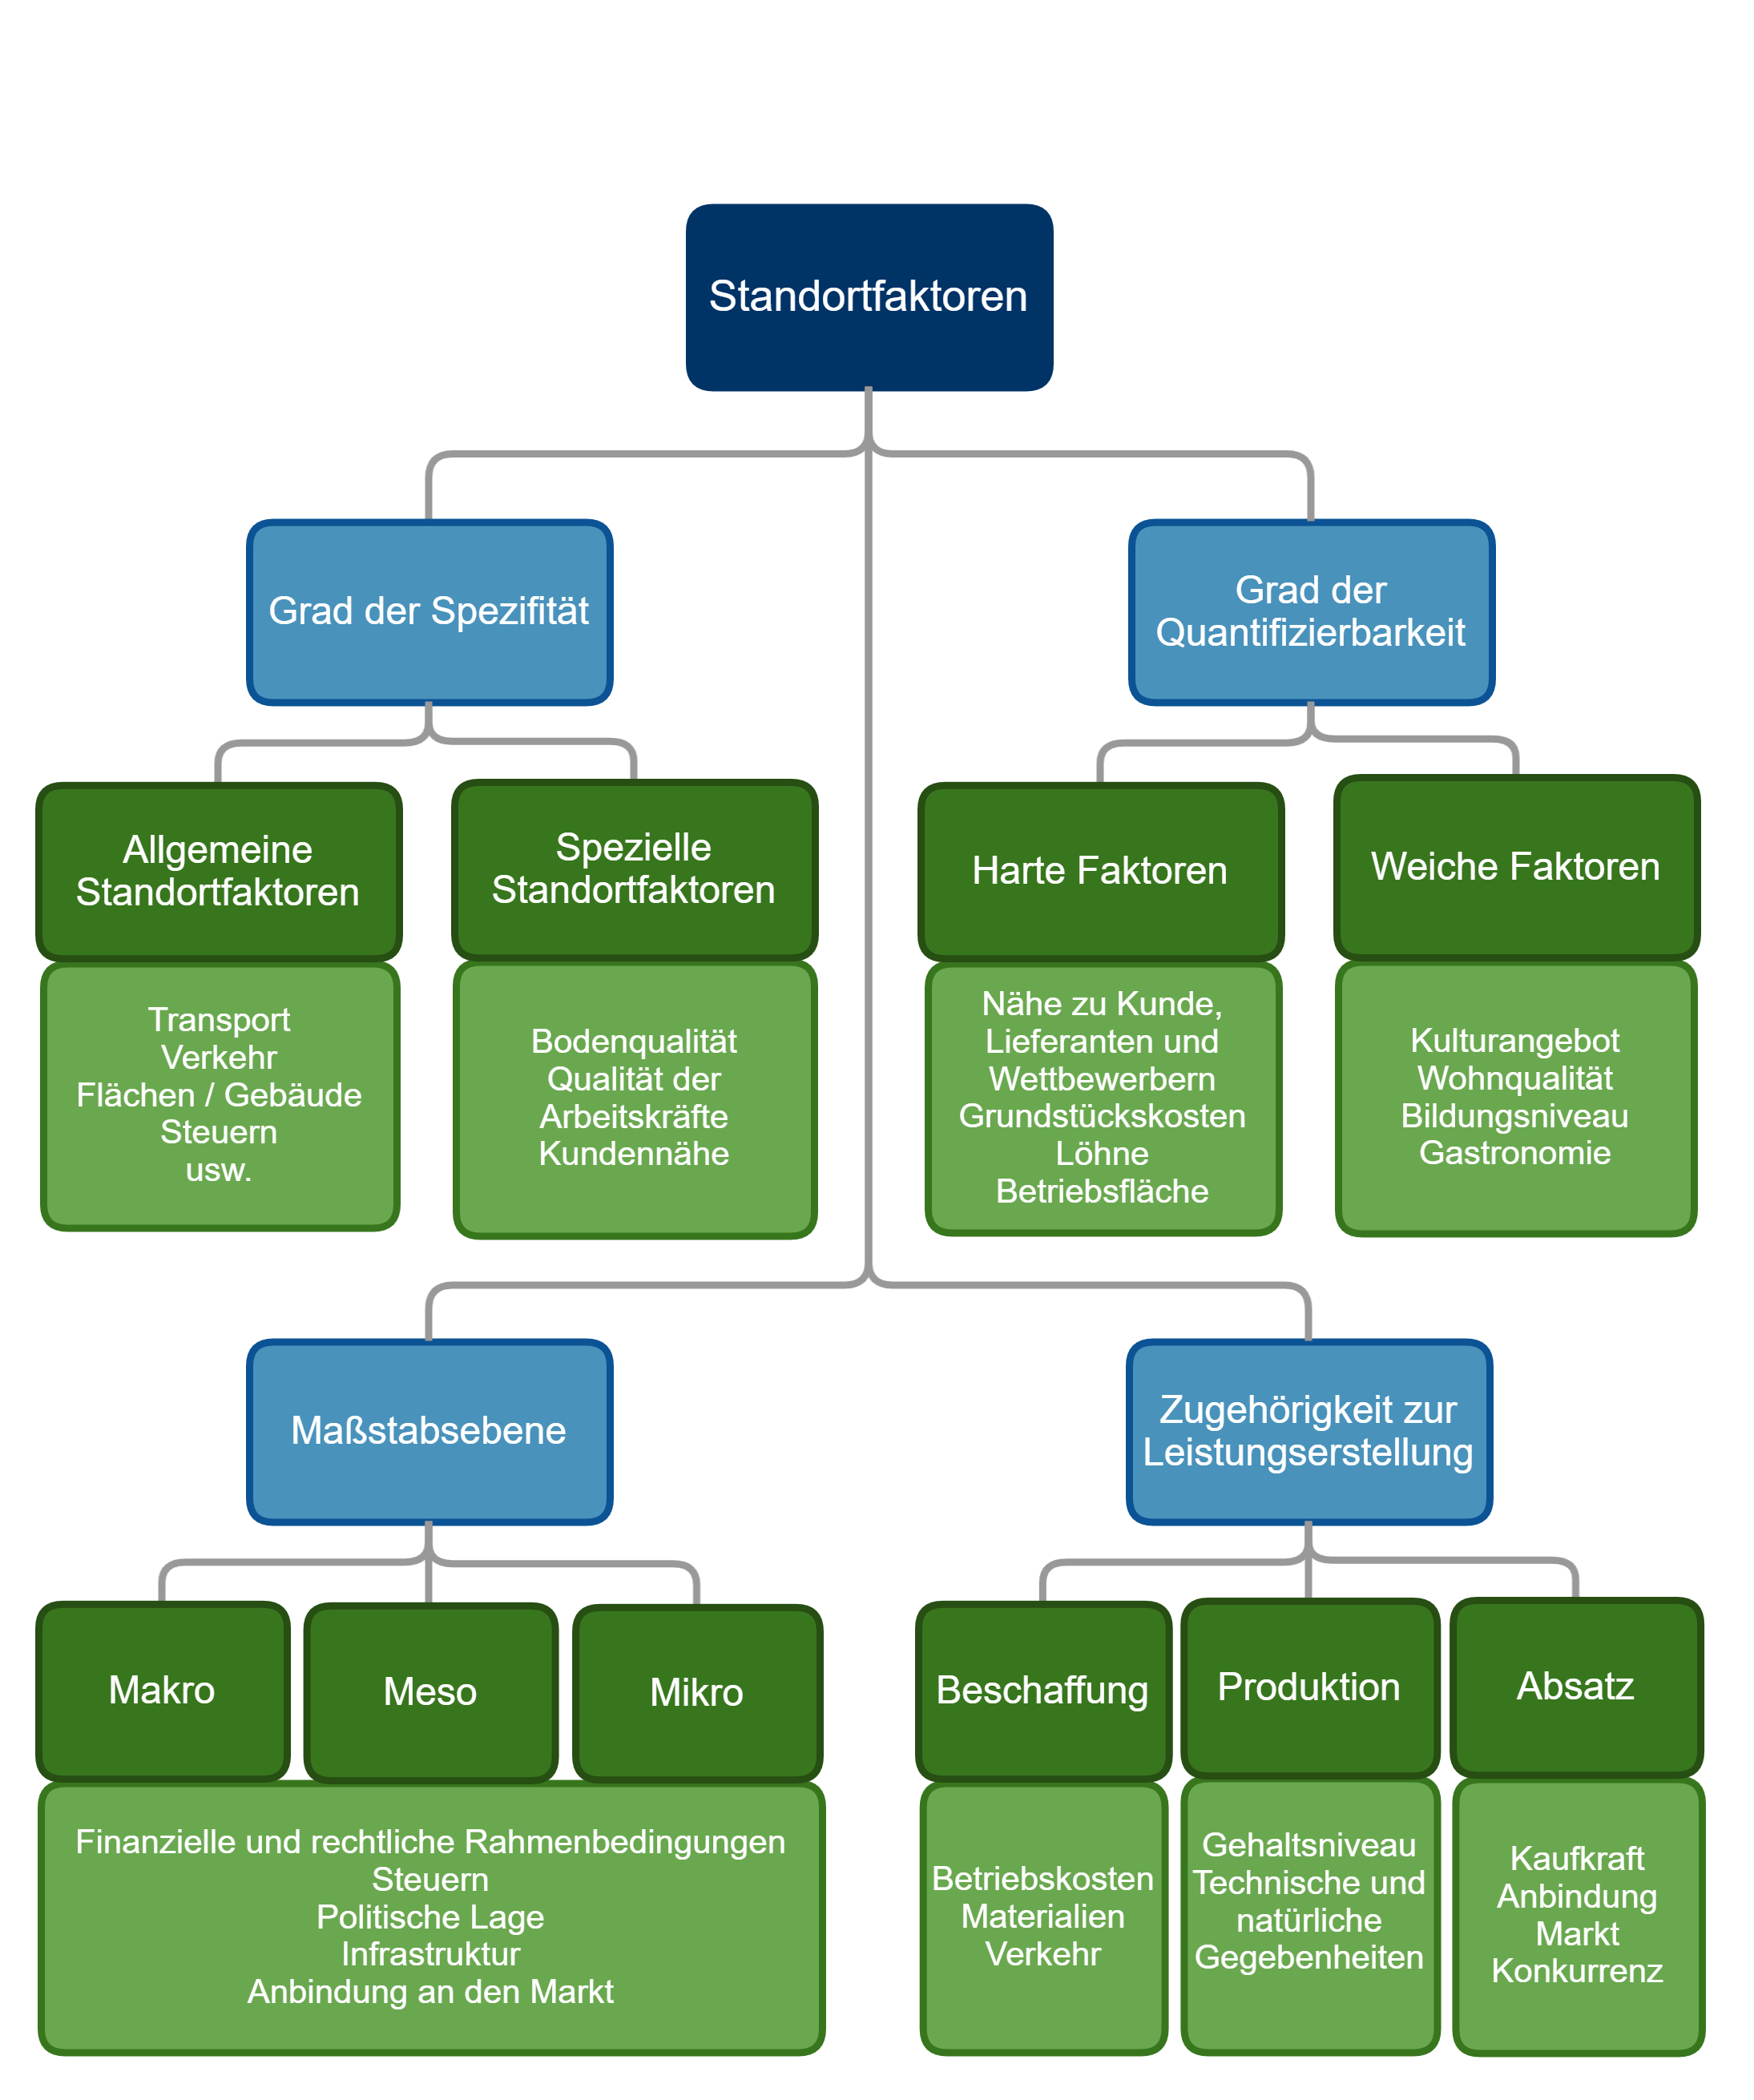
\includegraphics[scale=0.2]{resources/images/Standortfaktoren.png}
	\caption{Eigene Darstellung Standortfaktoren}
	\title{Standortfaktoren}
	\label{img:standortfaktoren}
\end{figure}

\newpage
Weitere zusätzlich relevante Aspekte können sein:
\begin{itemize}
	\item Zielgruppe: Wer sind die Kunden? Ist das Verkaufsmodell B2C oder B2B?
	\item Demografische Merkmale: Alter, Geschlecht und Wohnort der Kunden
	\item Sozioökonomische Betrachtung: Gibt es einen Zusammenhang zwischen Beruf, Bildungsstand oder Einkommen und dem Kaufverhalten?
	\item Psychografische Merkmale: Haben der Lebensstil, Werte, Motivation oder Ähnliches Einfluss auf das Kaufverhalten?
	\item Wettbewerbsdichte
	\item Preispolitik der Wettbewerber
	\item Größe des Einzugsgebiets
	\item Kaufkraftwerte des Gebiets
	\item Erreichbarkeit
	\item Mietpreise
	\item Attraktivität des Standortes
\end{itemize}

Obwohl Filialen geographisch aus betriebswirtschaftlicher Sicht Unternehmensstandorte sind, kann zwischen Filialplanung und Standortplanung unterschieden werden und dementsprechend werden andere Faktoren bei der Standortanalyse wichtiger oder hinzugezogen.
Für die Filialplanung zusätzlich relevant werden folgende Faktoren:

\begin{itemize}
	\item Bekanntheitsgrad, Markenstärke: Was zeichnet die eigene Marke aus? Was setzt sie ab?
	\item Freies Potential: Herrscht genug Nachfrage?
	\item Kannibalisierungs-Effekte: Ist der Standort zu nah an anderen, bestehenden Filialen?
	\item Logistikkosten: Kann ich Lieferwege und Lagerstandorte optimal nutzen?
\end{itemize}

Für eine einfache mathematische Standortanalyse können nun zunächst die Kategorien anhand der eigenen Marke als mehr oder weniger relevant bewertet und gewichtet werden.
Außerdem müssen die einzelnen Kategorien für jeden Standort bewertet werden. 
Die Bewertungen der Kategorien müssen nun mit der Gewichtung der Kategorie multipliziert werden, um die genaue Faktorbewertung des Standorts für jede Kategorie zu erhalten. 
Die Faktorbewertungen summiert ergeben nun Standortbewertung. 
Sind die Standortbewertungen tabellarisch aufgelistet und werden anschließend verglichen ist die Standortanalyse abgeschlossen.

\subsection{Standortplanung/ Filialplanung}
Bereits im vorherigen Kapitel erwähnt, wird zwischen der Standortplanung und der Filialplanung geringfügig unterschieden.
So legt die Filialplanung ihren Fokus auf mehrere in einem Filialnetz zusammengefasste Standorte, welche bei der Analyse berücksichtigt werden müssen.
Die Standortplanung konzentriert sich dagegen eher auf einzelne Standorte.

Beide Methoden verwenden jedoch in der vorher durchgeführten Standortanalyse herausgestellte Erkenntnisse, um die potenziellen Standorte einzuordnen und eine Entscheidung für die nächste Filialeröffnung zu treffen.

\subsection{Geodaten}
Geodaten sind strukturierte codierte Angaben zur quantitativen und qualitativen Beschreibung von natürlichen oder definierten Objekten der realen Welt. 
Geodaten vermessen die Welt und beschreiben geographische (Teil-)räume und Orte \footcite{geomarketing_geodaten}.

Geodaten werden in mehrere Typen klassifiziert und unterliegen definierten Standards, die sich am Markt durchgesetzt haben \footcite{gistandards.eu}.

So definiert die ISO 19115 einen Standard zur Beschreibung geographischer Informationen anhand von Metadaten \footcite{19115_iso}.
Wichtigste standardisierte Dienste sind unter anderem:

\begin{itemize}
	\item WMS: Web Map Service zum Teilen von Karten
	\item WFS: Web Feature Service zum Teilen von Feature-Daten
\end{itemize}

Zu den wichtigsten standardisierten Datenformaten zählen:

\begin{itemize}
	\item GeoJSON - JSON Format mit Geo-Spezifika
	\item KML - Keyhole Markup Language 
	\item GPKG - GeoPackage definiert vom Open Geospatial Consortium
\end{itemize}

Im Prototyp verwendete Formate sind GeoJSON für Features sowie einfache Bilder (PNG) der Hintergrundkarte.

\subsection{Marktdaten}
Marktdaten oder Marktinformationen beschreiben die individuelle regionale Charakteristik geographischer Gebiete oder Standorte mittels qualitativer Merkmale \footcite{geomarketing_marktdaten}.

Es gibt unternehmensinterne sowie externe Marktdaten.
Marktdaten können aus einem internen CRM-System stammen und über Umfragen, Marktforschung und Erhebungen als Primärdaten selbst erhoben werden oder aus staatlichen Statistiken sowie Branchen- und Wirtschaftsverbänden als Sekundärdaten eingeholt werden.

Im Prototyp verwendete Marktdaten sind aus Sekundärdaten erstellte Beispieldaten für Filialen und Gebiete.

\section{Geoinformationssysteme}
\label{sec:gis}
Geoinformationssysteme, kurz GIS, sind Informationssysteme zur Erfassung, Bearbeitung, Organisation, Analyse und Präsentation räumlicher Daten \footcite{geomarketing_gis}.  
Ähnlich anderer Informationssysteme besteht ein GIS aus Hardware (Computer, Server, Drucker etc.), Software mit Analyse-Tools (Zeichnen, Kalkulation) und räumlichen Daten (Koordinatensystem, Karten, Geometrien etc.). 
Gegebenenfalls wird die Liste um eine Verwaltungsebene ergänzt sobald ein Berechtigungskonzept für die Daten und Funktionen des GIS angewendet wird.
Erste GIS Systeme stammen aus den sechziger Jahren (Canada Geographic Information System \footcite{esri_cgis}). 
Zu den ersten Nutzern der Systeme gehörten vor allem Behörden und Universitäten, so wurden viele grundlegende theoretische Konzepte an der Harvard University von Professor Howard Fisher aufgestellt \footcite{gis_harvard_2005}.
Mittlerweile haben sich viele Web-GIS etabliert, hierbei wird das Informationssystem über eine Website veröffentlicht oder benutzt. 
Zu den größten Vertretern moderner Web-GIS zählen vor allem Google Maps, Bing Maps, OpenStreetMaps als OpenSource-Alternative oder etwas kleinere Anbieter wie HERE oder Yandex.Maps.
Kommerzielle Web-GIS bieten meist ein eingeschränktes Funktions-Set, was sie nicht als Produkt für individuelle Software-Lösungen für Firmen in Frage kommen lässt. Daher greifen viele Firmen auf kommerzielle Desktop-GIS zurück oder lassen sich ganz individuelle Systeme bauen, die aus Web- und Desktop-GIS bestehen.
Zu den bekanntesten GIS zählen Produkte von ESRI, Autodesk, Pitney Bowes oder CAIGOS. 

In der Geophysik wird die Erde nicht als Kugel, sondern als Ellipsoid bezeichnet \footcite{jung_figur_1956}.
Wenn man jedoch eine Karte elektronisch auf einem Bildschirm betrachtet, dann sieht man ein Rechteck und keine Anzeichen der Krümmung eines Globus.
Die Problematik der Projektion der Erde auf eine flache Darstellung hat über den Lauf der Jahre mehrere Lösungen produziert, die jedoch alle mit Koordinatensystemen und Projektionsrechnungen zu tun haben und bietet Stoff für ein eigenes Wissenschaftsfeld.
Aufgrund dessen versuchen die nächsten Zeilen, die Problematik und Anwendung im Prototyp kurz zu beschreiben.

In einem GIS muss die Projektion zwangsläufig enthalten sein und das bestenfalls für mehrere Projektionstypen.
Die meisten Web-Karten wie Google Maps oder Bing Maps benutzen die Projektion World Geodetic System 1984 (kurz WGS 84) mit dem Koordinatenreferenzsystem (engl. CRS) der European Petroleum Survey Group (kurz EPSG) 4326, welches Koordinaten in Grad darstellt \footcite{epsg.io_4326}.
OpenLayers hingegen benutzt standardmäßig WGS 84 mit EPSG 3857, welches Koordinaten in Metern zur Ursprungskoordinate darstellt \footcite{epsg.io_3857}.
Die Abbildung \ref{img:epsg.io} zeigt die Koordinaten eines Punktes in Berlin in beiden Koordinatenreferenzsystemen.

\begin{figure}[H]
	\centering
	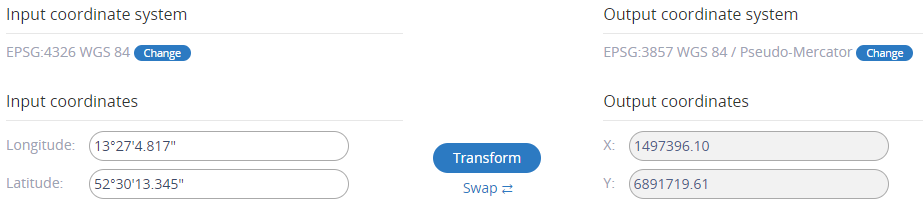
\includegraphics[scale=0.6]{resources/images/projection_epsg.png}
	\caption{Bildschirmaufnahme der Transformation  von EPSG 4326 zu EPSG 3857 von epsg.io \footcite{epsg.io_transform}}
	\label{img:epsg.io}
\end{figure}

Im Wesentlichen werden im Prototyp die oben beschriebenen Projektionen verwendet.
Die Geodaten der Filialen sowie der Zensusgebiete sind in EPSG 4326 erfasst und müssen dementsprechend vor der Darstellung transformiert werden.
Entsprechende Funktionen sind im Kapitel \ref{ch:implementierung} \glqqImplementierung\glqq beschrieben.

\section{Genutzte Technologie}
Für die prototypische Ausarbeitung des Modells wurde auf modernste Technologien und Frameworks zugegriffen. So wird als Karten-Framework /gls(ol) in der Version 6.4.3 verwendet sowie /gls(angular) in der Version 10.
Die Darstellung \ref{img:tech_stack} zeigt die genutzten Technologien als Grafik.

\begin{figure}[H]
	\centering
	
\includegraphics[]{resources/images/tech_stack.png}
	\caption{Eigene Abbildung des Technologie Stacks der Anwendung}
	\label{img:tech_stack}
\end{figure}

OpenLayers bietet ein breites Portfolio an Funktionen und Features passend für sämtliche Anforderungen realer Geo-Informationssysteme, die in der Praxis verwendet werden. 
Im Bezug auf die prototypische Anwendung dieser Arbeit sind vor allem die Unterstützung der Darstellung von Punkten (Filialen) und der Zensusgebiete in GeoJSON-Format auf verschiedenen Layern notwendig sowie die einfache Konfigurierbarkeit von Karten-Interaktionen, wie zum Beispiel das Platzieren, Verschieben und Editieren von Punkt-Objekten (Filialen) auf der Karte.

Weiterführend soll die Anwendung schnell, kompakt und modern sein, um die Relevanz aus Gründen der Performance auf dem Markt gewährleisten zu können. 
Daher erfolgt die Umsetzung mit dem auf TypeScript basierenden Framework Angular. Besonderes Augenmerk liegt hierbei im Prototyp eigentlich nur auf der simplen, kompakten und schnellen Auslieferung eines Web-Servers als Host der Anwendung. Zu den für die weiterführende Entwicklung relevant werdenden Features des Frameworks zählen eine große Community, einen fortlaufenden Support sowie eine fortlaufende Entwicklung durch Google, die Verwendung von TypeScript, einem Superset von JavaScript mit verbesserter Funktionalität und sämtlichen Features, die für Entwicklung einer effizienten und anspruchsvollen Single-Page-Webanwendung benötigt werden.  \clearpage
\chapter{Konzept}
\label{ch:concept}
Die Algorithmen und Prozesse einer Filialplanung geben sehr gut einen allgemeinen Anwendungsfall moderner GIS wieder. 
Neben einer einfachen Hintergrundkarte sind die Mitarbeiter auf Zeichenwerkzeuge, Geo-Daten-Anzeige, thematische Karten und Kennzahlen Berechnungen angewiesen, um akkurate und fundierte Prognosen und Planungen treffen zu können.
Viele theoretische Konzepte und Prozesse passieren hierbei im Hintergrund und sind nicht direkt ersichtlich.

In den folgenden Kapiteln werden Prozesse der Standortanalyse beschrieben und der Fokus auf das Gravitationsmodell von Huff als Algorithmus zur Bestimmung des Marktanteils gelegt.
Ebenso wird die daraus entstehende Architektur des Prototyps vorgestellt.

\section{Algorithmus und Prozesse}
Die Filialplanung ist ein Prozess, der sich aus mehreren Teilprozessen zusammensetzt. 
Einer dieser Teilprozesse ist die Standortanalyse bezogen auf Filialen.
Die Wahl eines Standortes ist keinesfalls immer eindeutig und anhand des potenziellen Umsatzes der neuen Filiale zu erkennen.
So kann es zum Beispiel durchaus sinnvoll sein eine Filiale trotz möglicher Kannibalisierung anderer eigener Filialen dennoch zu eröffnen, weil dies gleichzeitig zu Umsatzeinbußen bei Konkurrenzfilialen führt. 
Der eigene Marktanteil und Gesamtumsatz ist der entscheidende Faktor bei der Filialplanung.
Durch die Anwendung ausgewählter Algorithmen gilt es also folgende Leitfrage zu beantworten:

Wo befindet sich der ideale Standort, um eine neue Filiale zu eröffnen?

Um diese Frage fundiert beantworten zu können, ergeben sich mehrere vorliegende Fragen:

Wo kann ich überhaupt eine neue Filiale eröffnen?\\
Was ist mit meinen Konkurrenten, was ist mit Kannibalisierung meiner eigenen Filialen?\\
Wie kann ich folglich also sicherstellen, dass sich mein Gesamtumsatz durch die Neueröffnung steigert?

Die Suche nach dem idealen Standort beginnt zunächst bei der Eingrenzung möglicher Standorte.
Im modernen Stadtbild ist die Anzahl freier Standorte begrenzt.
Meist bestimmt das Angebot die Möglichkeiten.\\
Existiert nun eine Liste möglicher Standorte, muss für jeden Standort der Einfluss auf das bestehende Filialnetz erfasst werden.
Das bestehende Netz kann nur eigene Filialen beinhalten, um die Kannibalisierung meines eigenen Netzes durch eine Neueröffnung zu analysieren, oder Konkurrenzfilialen und Lager einschließen, um den Einfluss auf den Gesamtmarkt zu berechnen.\\
Wichtige Parameter für die Berechnung des Marktanteils der Filialen im Netz sind Attraktivität, Nähe zu Zielgruppen und die Entfernung zu anderen Filialen.\\
Über das Huff-Modell kann die Auswirkung auf den Marktanteil aller Standorte berechnet werden.
Im Folgenden wird das Modell und zugehörige Komponenten im Detail vorgestellt.

Gravitationsmodelle in der Ökonomie leiten sich vom newtonschen Gravitationsmodell ab und beschreiben den Einfluss der Marktgrößen verschiedener Länder (meist das BIP) und der Entfernung zwischen beiden auf die bilateralen Handelsströme zwischen den Ländern.\\
Das \textit{Huff-Modell} (engl. Huff Gravitation Model) ist ein mathematisches Modell zur Abgrenzung und Segmentierung von Marktgebieten, welches sich direkt aus deterministischen Modellen zur Anwendung von Gravitationsmodellen in der Bestimmung von Einzugsgebieten im Einzelhandel von William J. Reilly und P.D. Converse ableitet \footcite{reilly_law_1931} \footcite{converse_new_1949}.
Das Modell bestimmt die Wahrscheinlichkeit, mit der Kunden einen Standort (Filiale, Einkaufszentrum) in Abhängigkeit von Distanz und Attraktivität aufsuchen \footcite{arcgis_funktionsweise_huff}. 
Die Formel wird im allgemeinen wie folgt dargestellt:

\begin{equation}
	P_{i j}=\frac{A_{i}^{\alpha} / D_{i j}^{-\beta}}{\sum_{i=1}^{n}\left(A_{i}^{\alpha} / D_{i j}^{-\beta}\right)}
\end{equation}

Dabei gilt:

\( P_{i j} \) = die Wahrscheinlichkeit, mit der Kunde j in Filiale i einkauft;\\
\( A_{i} \) = ein Maß für die Attraktivität der einzelnen Filiale i;\\
\( D_{i j} \) = die Entfernung von Kunde j zu Filiale i;\\ 
\( \alpha \) = ein Exponent, der auf die Attraktivität angewendet wird, um die Wahrscheinlichkeit von attraktiveren Standorten zu vergrößern;\\ 
\( \beta \) = ein Exponent, der auf die Entfernung angewendet wird, um die Wahrscheinlichkeit von entfernten Standorten zu verringern;\\
n = die Anzahl der Filialen.

Die Wahrscheinlichkeiten werden nun auf der Karte als Punkte dargestellt, die rund um den Standort platziert werden. 
Die Punkte der selben Wahrscheinlichkeiten werden zu Isowahrscheinlichkeitslinien verbunden. 
So entstehen zu jedem Standort verschiedene Gravitationsebenen, die farblich gekennzeichnet werden. 
Die Beeinflussung der verschiedenen Gravitationsebenen führt zu mehreren Farbverläufen, die ein komplexes Bild der Standort Landschaft bilden.
In seiner einfachsten Form berücksichtigt das Modell nur die Distanz und eine simple Kennzahl der Attraktivität (zum Beispiel in Form eines Rankings) für die Wahrscheinlichkeitsberechnung. 
Hierzu wird zunächst ein maximaler Einflussbereich der Filialstandorte definiert. 
Dieser Bereich stellt die Grundlage der Berechnungen dar und muss deswegen bekannt und mit berechenbaren Kennzahlen gefüllt sein.
Zur Bestimmung des Bereiches können einfache geografische Abstände oder Gebiete benutzt werden, wie zum Beispiel eine Berechnung auf Grundlage Berlins als Einflussbereichs.
Vor Allem aber kommen zeitliche oder örtliche Parameter zum Einsatz.
So macht es aus wirtschaftlicher Sicht viel mehr Sinn das Gebiet anhand von Fahrzeitzonen zu berechnen.
So würde ein potenzieller Kunde aus Brandenburg wahrscheinlich auch in einer Filiale in Berlin einkaufen gehen, wenn diese attraktiver, örtlich näher oder besser zu erreichen ist.
Berechnet wird also ein Einzugsbereich, um die Filiale herum.
Ob dies nun eine maximale Fahrtzeit von 30 Minuten ist oder eher eine maximale Distanz von 30 Kilometern, ist auf die einzelne Filiale oder den gewählten Standard der Berechnung zurückzuführen.

Um das Modell korrekt kalibrieren zu können, genauer gesagt die Parameter $\alpha$ und $\beta$ empirisch bestimmen zu können, müssen folgende Schritte befolgt werden \footcite{huff_calibrating_2008}:

\begin{itemize}
	\item Abgrenzung des Erhebungsgebiets
	\item Unterteilung des Erhebungsgebiets in Untergebiete
	\item Zentroiden der Gebiete festlegen
	\item Alle konkurrierende Einrichtungen identifizieren und Koordinaten erfassen
	\item Entfernungen zwischen den Zentroiden aller Gebiete und aller Einrichtungen berechnen
	\item Spezifizieren aller Eigenschaften zur Kundenbeeinflussung
	\item Wirtschaftliche, soziale und demografische Daten für Gebiete angeben
	\item Studie durchführen für die Frequenz in welcher Kunden Einrichtungen besuchen
\end{itemize}

Der Parameter $\alpha$ sollte nun normalerweise aus den Studienergebnissen abgeleitet werden, indem für die Abhängigkeit der Attraktivität einer Filiale mit der wirklichen Besucherzahl der Filiale ein Faktor bestimmt wird.
Im Prototypen wird diese Zahl auf 1,5 festgesetzt und somit der Attraktivität einer Filiale eine erhöhte Wichtigkeit beigemessen.\\
Weiterführend muss nun auch noch bestimmt werden wie und ob sich das Potenzial über den Verlauf der Distanz des Einzugsbereiches verändert, dieses Potential äußert sich im Modell über den Parameter $\beta$.
Bleibt das Potenzial konstant, würde dies bedeuten die Kunden in den äußeren Bereichen des Gebiets kommen mit der gleichen Wahrscheinlichkeit in die Filiale wie die Kunden in den unmittelbar angrenzenden Bereichen.
Aber gegenteilig wäre ein linear abnehmendes Potenzial wahrscheinlich ebenso nicht vollständig realitätsgetreu, da Kunden ab einer Distanz, die zu groß für den Fuß-Weg wäre, eher das Auto oder den öffentlichen Nahverkehr wählen und dann eventuell direkt zu einer attraktiveren Filiale weiter weg fahren würden. 
Daher kann als grundlegende Distanzfunktion quasi eine beliebig komplizierte Formel gewählt werden.
Aus Gründen der Vereinfachung und Demonstration wird für den Prototyp eine einfache linear abnehmende Distanzfunktion gewählt, welche den Parameter $\beta$ auf 1,5 festlegt.\\

Nachdem nun zunächst die Potenzialberechnung für eine einzelne Filiale anhand der beschriebenen Parameter und Funktionen erfolgen konnte gilt es nun das Potenzial in einem bestehendem Filialnetz zu berechnen.
Als Ergebnis wird hierbei eine Wahrscheinlichkeitsberechnung für sämtliche Filialen des Netzes erwartet, sodass jedem Feld des summierten Gesamt-Einzugsgebietes einen Wahrscheinlichkeitswert zugeordnet werden kann, der beeinflusst von sämtlichen anderen Filialen des Netzes, für jede Filiale des Netzes unterschiedlich sein kann und dementsprechend eingefärbt werden kann.
Das Endergebnis zeigt somit die beschriebene farbliche Gravitationskarte.

\section{Architektur}
Die Architektur der Anwendung ergibt sich hauptsächlich aus den fachlichen Anforderungen und technischen Voraussetzungen. 

Das Diagramm \ref{img:components_diagram} zeigt die Komponenten der Anwendung im Zusammenspiel in einer eigenen Darstellung.

\begin{figure}[H]
	\makebox[\textwidth][c]{
	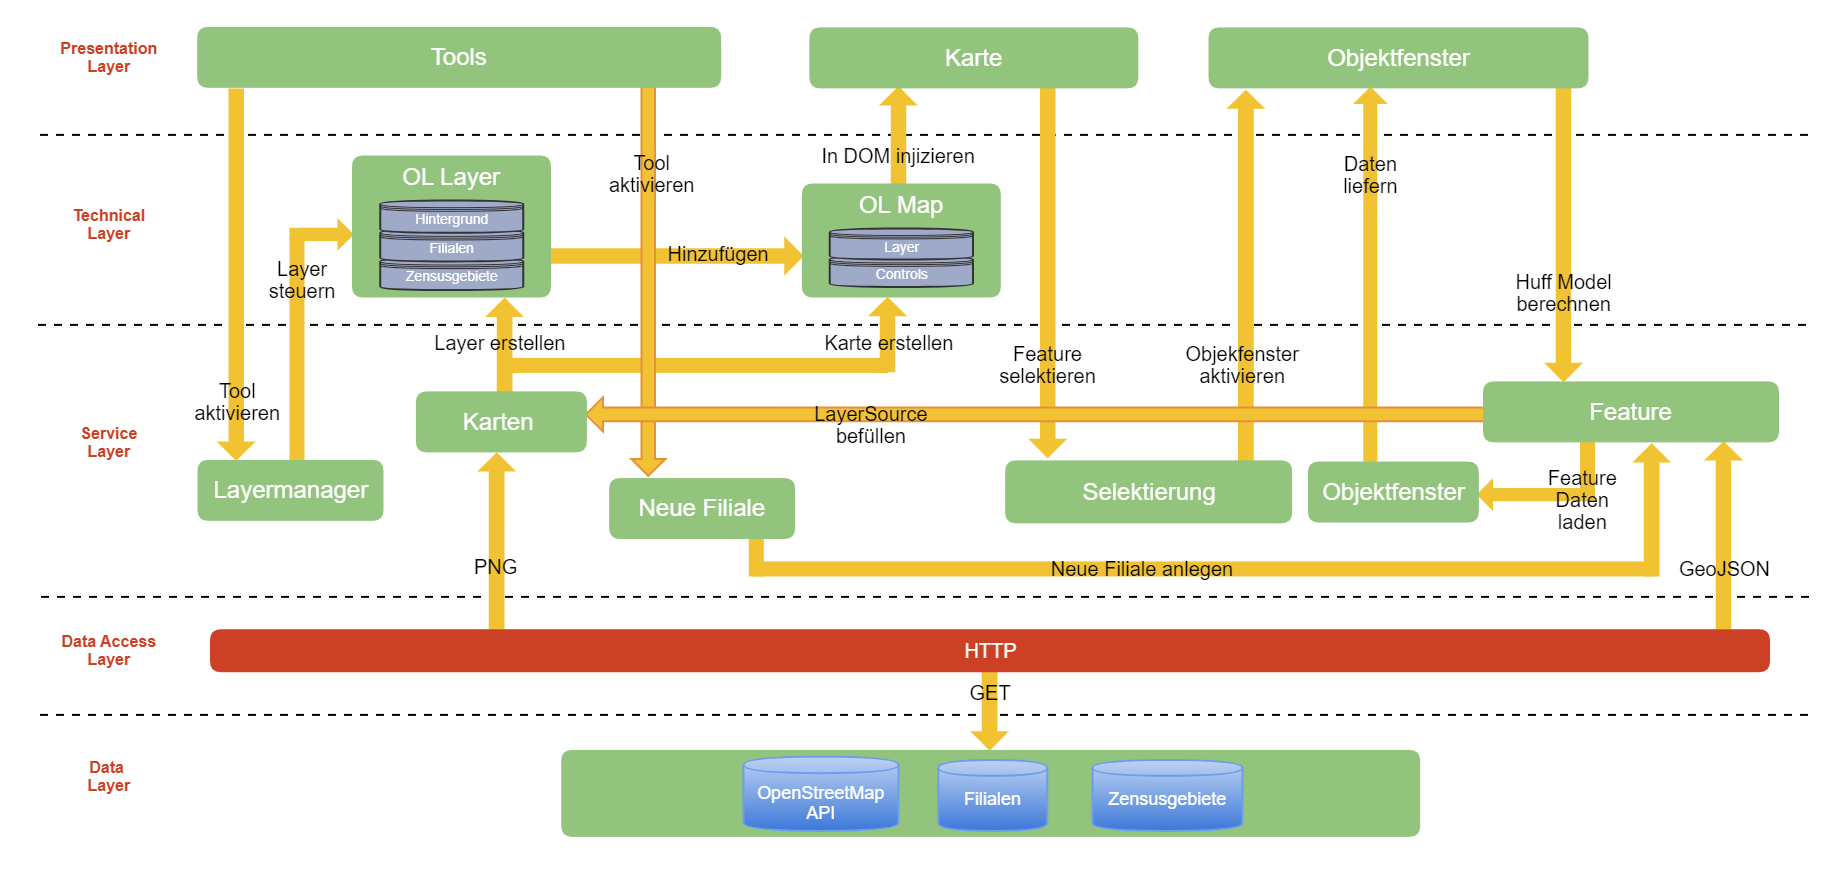
\includegraphics[width=1.0\textwidth]{resources/images/architecture.png}}
	\caption{Komponentendiagramm der Anwendung in eigener Darstellung}
	\label{img:components_diagram}
\end{figure}

Die Anwendung baut im wesentlichen auf vier Komponentengruppen auf:

\begin{itemize}
\item Angular Komponenten
\item Angular Services
\item OpenLayers Karte und Layer
\item Geo-Daten
\end{itemize}

OpenLayers als GIS-Software bildet hierbei den Kern in Form der Karte.
Die Karte bietet an sich bereits einen großen Teil der GIS-Werkzeuge, die für die Anwendung benötigt werden.
Die Karte stellt die Layer und deren Sourcen in der richtigen Projektion dar und bietet die Selektierungs-Interaktion der einzelnen Features.
Sie sorgt also dafür, dass die ovale Weltkarte auf den flachen Bildschirm projiziert wird und der Klick auf eine Pixel-Koordinate des Bildschirmes umgerechnet eine geografische Koordinate widerspiegelt.
Die Karte wird in der Anwendung im BaseMap-Service mit Parametern erstellt und in der OpenLayersMap-Komponente in den DOM injiziert. 

Der Karte werden drei Layer hinzugefügt:

\begin{itemize}
\item Hintergrund-Layer
\item Filial-Layer
\item Zensusgebiete-Layer
\end{itemize}

Fachlich betrachtet kann der Hintergrund-Layer auch als Hintergrundkarte bezeichnet werden, technisch ist er jedoch ebenso ein Layer wie die Filialen und Gebiete. 
Die Layer werden im BaseMap-Service erstellt und der Karte in der OpenLayersMap-Komponente hinzugefügt.
Zu den Layern gehören entsprechende Sources, über die Features in den Layer und somit dargestellt werden können.

Der Hintergrund-Layer ist ein Kachel-Layer (Englisch: Tile-Layer).
Der Layer wird durch ein Gitter (Englisch: Grid) in einzelne Kacheln eingeteilt, die alle einzeln mit Bildern befüllt werden.
Dies ist ein Optimierungsschritt, der den Datentransfer reduziert sowie die Renderingzeit und -performance verbessert.
Die Kachelbilder werden über Http-Requests an die OpenStreetMap-API geladen.

Die beiden Feature-Layer der Filialen und Gebiete sind Vektor-Layer (Englisch: Vector-Layer).
Die jeweiligen Sources der Layer lesen die Features über lokale GeoJSON-Dateien im Feature-Service ein und befüllen den Layer im BaseMap-Service mit den Sourcen.

Nun sind die Features über ihre Layer auf der Karte zu sehen und können über eine Selektions-Interaktion in der Karte ausgewählt werden.
Über den SelectFeature-Service wird daraufhin das Objektfenster aktiviert, welches Informationen über das Feature enthält und die Berechnung des Huff-Modells für die selektierte Filiale starten kann.
Die Daten des Features werden über den Objektfenster-Service in das Objektfenster injiziert.

Über die Tool-Komponente kann eine neue Filiale auf die Karte gesetzt werden und die Layer gesteuert werden.

Sobald eine neue Filiale auf der Karte gesetzt ist wird über den Neue-Filiale-Service ein weiteres Feature in die Filiale-LayerSource geladen und über das Objektfenster kann nun die Berechnung des Huff-Modells gestartet werden.

Über das LayerManager-Tool kann im LayerManager-Service die Sichtbarkeit und Reihenfolge der Layer gesteuert werden.
 \clearpage
\chapter{Implementierung}
\label{ch:implementierung}
Das Kapitel Implementierung erfasst die technische Dokumentation des erarbeiteten Prototyps.
Im Detail werden in den folgenden Seiten die technische Umsetzung des in Kapitel \ref{ch:concept} entworfenen Konzepts beschrieben. 
Beschriebene Funktionalitäten werden mit Bildausschnitten unterstützt.

\section{Prototyp}
Die Anwendung wurde als Angular Projekt mittels der Angular CLI erstellt. 
Über den CLI Befehl 

\begin{lstlisting}[language=bash, caption={Erstellen eines neuen Projektes}]
$ ng new gravitationsmodel
\end{lstlisting}

generiert die CLI ein kompilierbares und ausführbares Angular Projekt mit essentiellen Abhängigkeiten und Strukturen.
Angular verwendet standardmäßig NPM als package manager.
Eine \emph{package.json}, welche sämtliche Abhängigkeiten dokumentiert, wird bereits mit erstellt.
Um das Setup abzuschließen müssen weitere Abhängigkeiten in Form von \emph{npm packages} installiert werden.
Über den Befehl 

\begin{lstlisting}[language=bash, caption={Hinzufügen des OpenLayers Pakets}]
$ ng add ol
\end{lstlisting}

fügt die CLI automatisch das Paket von OpenLayers hinzu und für die korrekte Typisierung in TypeScript das notwendige \emph{types} Paket für OpenLayers hinzu.

Nachdem die technischen Voraussetzungen geschaffen sind kann mit der Implementierung begonnen werden.
Auch hierbei bietet die CLI Unterstützung in Form von \emph{Scaffolding} Befehlen.

\begin{lstlisting}[language=bash, caption={Angular schematic Befehl zum Erstellen}]
$ ng generate <schematic> [name]
\end{lstlisting}

generiert Komponenten, Services, Models, Klassen und weitere Code-Gerüste durch den passenden Präfix-Parameter und Namen.
Angular Komponenten bestehen meist aus einer TypeScript-Klasse (\emph{.component.ts}), einem Template (\emph{.component.html}) sowie Dateien für Styling (\emph{.css} oder \emph{.scss}) und Tests (\emph{.component.spec.ts}).

\begin{lstlisting}[language=bash, caption={Erstellen der Objektfensterkomponente}]
$ ng generate component objektfenster
\end{lstlisting}

erstellt \emph{objektfenster.component.ts}, \emph{objektfenster.component.html} sowie \emph{objektfenster.scss} und \emph{objektfenster.component.spec.ts} Dateien.

Mit Hilfe der CLI lassen sich so die Code-Gerüste schnell erstellen und die CLI übernimmt sogar die in Angular nötige \emph{Dependency Injection} indem neue Komponenten direkt in der entsprechenden \emph{.module.ts} deklariert werden \footcite{angular_cli}.

Ebenfalls im Zuge der Projekterstellung über die CLI werden Konfigurationsdateien angelegt, die wichtige Einstellungen zum Kompilieren, Bau, Start und Hosten (engl. host) der Anwendung enthalten.

Die Anwendung kann nun über 

\begin{lstlisting}[language=bash, caption={Starten der Anwendung}]
	$ ng serve
\end{lstlisting}

gestartet werden.
Der Befehl kompiliert, baut und startet die Anwendung über einen lokalen Webserver.
Über \emph{localhost:4200} kann die Anwendung im Browser aufgerufen werden.

Der Kern der Anwendung ist eine Karte mit der interagiert wird.
Um diese darzustellen, muss zunächst ein OpenLayers Map-Objekt erstellt und in den DOM eingehängt werden \footcite{openlayers_map}.
Dies geschieht in der OpenLayersMap-Komponente und dem BaseMap-Service.
Über das bereits installierte OpenLayers Paket wird das Map-Objekt importiert und initialisiert.

\begin{lstlisting}[language=JavaScript, caption={Erstellung der Karte}]

	const targetId = 'map';
	const longitude = 13.451338;
	const latitude = 52.503707;
	const zoomLevel = 11;
	
	const coordinate = fromLonLat([longitude, latitude]);
	
	const view = new View({
		center: coordinate,
		zoom: zoomLevel
	});
	
	const map = new Map({
		target: targetId,
		layers: [],
		view,
	});


\end{lstlisting}

Die Karte wird mit der notwendigen Id des HTML-Elements, in welchem die Karte angezeigt werden soll, und einem View initialisiert.
Das View-Objekt besteht aus einer Center-Koordinate und der initialen Zoomstufe und stellt den Begrenzungsrahmen (engl. Bounding Box) der Karte dar.
Zu beachten ist ebenfalls hierbei die Transformation der Koordinaten von EPSG:4326 in das in OpenLayers standardmäßig genutzte EPSG:3857 über die Funktion \emph{fromLonLat}.
Die Karte wird ebenfalls mit Standard-Interactions und Standard-Controls initialisiert jedoch sind noch keine Layer hinzugefügt.
Somit ist jetzt auch noch nichts auf der Karte zu sehen und lediglich bereits erwähnte Controls und Interactions sind sichtbar und bedienbar.
Zu den Controls zählen:

\begin{itemize}
	\item Zoom
	\item Rotate (Unsichtbar bei Rotation 0)
	\item Attribution
\end{itemize}

Sowie Interactions:

\begin{itemize}
	\item Drag rotate
	\item Drag pan
	\item Drag zoom
	\item Double click zoom
	\item Mouse wheel zoom
	\item Pinch rotate (Touchscreen)
	\item Pinch zoom (Touchscreen)
	\item Keyboard pan
	\item Keyboard zoom
\end{itemize}

Als nächstes wird der Hintergrundkarten-Layer hinzugefügt.
Hierzu wird ein neuer Tilelayer initialisiert, eine neue Layer-Quelle (engl. Source) hinzugefügt und der Layer der Karte hinzugefügt.

\begin{lstlisting}[language=JavaScript, caption={Erstellung der Hintergrundkarte}]
	
	const backgroundLayer = new TileLayer();
	backgroundLayer.setSource(new OSM());
	backgroundLayer.set('name', 'Hintergrund');
	
	map.addLayer(backgroundLayer);	
	
\end{lstlisting}

Der Hintergrundkarten-Layer ist ein Kachel (engl. Tile) Layer, da dies die Datenabfrage an den Kartendienstleister, in diesem Fall OpenStreetMaps, reduziert und eine optimale Render-Performance erzeugt.
Ein Tile-Layer teilt den Kartenausschnitt in ein Gitter (engl. Grid) aus vielen kleinen Kacheln ein.
Jeder dieser Kacheln setzt ihren eigenen Http-Request an den in der Source angegeben Provider mit den Kachel-Koordinaten und Zoom-Stufe als Parameter ab und bekommt einen Kartenausschnitt in PNG-Format zurück.
Die einzelnen Bilder werden dann im Cache des Browsers gespeichert und sorgen somit für verminderten Datentransfer sowie schnelles Laden bei erneutem Aufruf.
OpenLayers bietet für OpenStreetMap sowie Bing Maps eigene Source-Objekte, welche für Bing nur noch einen API-Key benötigt.
Um den Layer später einmal einfach identifizieren zu können, wird dem Layer noch eine Name-Eigenschaft zugewiesen.

Nach der Hintergrundkarte müssen nun noch Layer für die Filialen sowie die Zensusgebiete implementiert werden.
In der OpenLayersMap-Komponente werden dazu zwei neue Layer mit passenden Source-Objekten angelegt.

\begin{lstlisting}[language=JavaScript, caption={Erstellung der Filial- und Gebietelayer}]

	const filialLayer = new VectorImageLayer({
		visible: true,
		zIndex: 2
	});	
	filialLayer.set('name', 'Filialen');
	filialLayer.setSource = new VectorSource({
		format: this.geoJSONFormat,
		strategy: bbox	
	});

	const gebieteLayer = new VectorImageLayer({
		visible: true,
		zIndex: 1
	});
	gebieteLayer.set('name', 'Gebiete');
	gebieteLayer.setSource = new VectorSource({
		format: this.geoJSONFormat,
		strategy: bbox	
	});

	map.addLayer(filialLayer);
	map.addLayer(gebieteLayer);
\end{lstlisting}

Bei der Initialisierung der Layer muss die Z-Ebene der Filialen höher sein, da sie später in der Anwendung über den Gebieten liegen sollen und nicht von diesen überlagert werden sollen.
Bei VectorSources kann zwischen den Ladestrategien Tile und Bounding Box entschieden werden.
Sie bestimmt wann neue Features auf der Karte geladen und angezeigt werden sollen.
Bei der Tile-Strategie wird wie bei der Hintergrundkarte der Kartenausschnitt in ein Kachelgitter unterteilt und bei der Bounding Box Strategie wird der gesamte Kartenausschnitt (engl. Bounding Box) gewählt. 
Bei besonders vielen Daten sollte auf die Tile-Strategie zurückgegriffen werden aber im Prototypen reicht die Bounding Box Strategie vollkommen aus.

OpenLayers definiert standardmäßig für jeden Vector Layer einen Stil, der die einzelnen Features je nach Geometrietyp auf der Karte darstellt. 
Soll dieser Stil geändert werden, muss auf dem Layer ein neuer Stil definiert werden.
Dies kann über ein statisches Style-Objekt erfolgen oder über eine dynamische Style-Funktion.

\begin{lstlisting}[language=JavaScript, label={code:filialStyle}, caption={Erstellen des Filialstyles}]
	
	const filialStyle = new Style({
		image: new Icon({
			color: '673ab7'
		}),
		text: new Text({
			fill: new Fill({
				color: 'FFFFFF'
			})	
		})
	});
	
	const filialStyleFunction = (feature, resolution) => {
		if (feature.get('selected') === true) {
			filialStyle.getImage()
			.setSource('assets/geometries/icons/PIN_selected.svg');
		} else {
			filialStyle.getImage()
			.setSource('assets/geometries/icons/PIN.svg');
		}
		filialStyle.getText().setText(feature.getId().toString());
		return filialStyle;
	}
	
	filialLayer.setStyle(filialStyleFunction);

	
\end{lstlisting}

Nun werden realistische Geo- sowie Marktdaten benötigt.\\
Die Filialen sind einfache Koordinaten im Raum Berlin.
Ein Testdatensatz mit 97 Koordinaten wurde über geojson.io \footnote{\href{geojson.io}{geojson.io}} angelegt.
Die Koordinatenliste wird bereits in GeoJSON angelegt und die Einträge müssen lediglich um eine Id, Anzahl der Parkplätze sowie die Verkaufsfläche der Filiale ergänzt werden.\\
Ein Testdatensatz mit 1220 Zensusgebieten des Geoportals Berlin \footcite{geoportal_berlin} wurde über das ArcGIS Hub \footcite{arcgis_verkehrszellen} heruntergeladen.
Die Gebiete werden ebenfalls bereits in GeoJSON exportiert.
Da es sich jedoch um zu viele Einträge für eine manuelle Ergänzung der Marktdaten handelt, werden Marktdaten für die einzelnen Gebiete beim einlesen der Datei ergänzt.

Die Datensätze werden über das Feature Format GeoJSON in OpenLayers eingelesen und in eine FeatureCollection (bei einzelnen Daten in ein Feature) umgewandelt, welche der jeweiligen Layer Source hinzugefügt wird.

\begin{lstlisting}[language=JavaScript, caption={Laden der GeoJSON-Dateien der Filialen und Gebiete}]

		this.http.get('../assets/filialen.json').subscribe(value => {
			const readFeatures = this.geoJSONFormat.readFeatures(value);
			readFeatures.forEach(feature => {
				feature.setId(feature.get('id'));
				feature.set('type', FeatureTypeEnum.FILIALE);
			});
			filialLayerSource.addFeatures(readFeatures);
		});

		this.http.get('../assets/zensusgebiete.json').subscribe(value => {
			const readFeatures = geoJSONFormat.readFeatures(value);
			readFeatures.forEach(feature => {
				feature.setId(feature.get('id'));
				feature.set('type', FeatureTypeEnum.ZENSUSGEBIET);
			});
			gebieteLayerSource.addFeatures(readFeatures);
		});
		
	}		
	
\end{lstlisting}

Es handelt sich bei den Filial- sowie Gebietsdaten um fiktionale Daten, jedoch sollten diese einen repräsentativen Charakter haben und möglichst nah an realistischen Marktdaten gewählt werden.
Als Referenz der Parkplätze und Verkaufsfläche dienen Werte der Statistik "Entwicklung der durchschnittlichen Verkaufsfläche der Lebensmittel-Discountmärkte Lidl in Deutschland in den Jahren 2009 bis 2019 (in Quadratmetern)" von handelsdaten.de \footcite{handelsdaten_lidl} sowie die Anlage zu Nummer 51.11 der Verwaltungsvorschrift zu Landesbauordnung Nordrhein-Westfalen \footcite{bauo_5111}.
Aus den Quellen lässt sich eine durchschnittliche Verkaufsfläche von 898 Quadratmetern sowie 1 Parkplatz pro 10 Quadratmetern Verkaufsfläche erschließen.
Um den Filialen verschiedene Verkaufsflächen und Parkplätze zuzuordnen wurden Zufallszahlen im Bereich 798 bis 998 für die Verkaufsfläche gewählt sowie die sich daraus ergebende Anzahl der Parkplätze.\\
Bei den Marktdaten der Gebiete handelt es sich um Angaben zu Anzahl der Einwohner, durchschnittliche Kaufkraft und durchschnittliche Ausgaben für Lebensmittel pro Gebiet.
Als Referenz für die Marktdaten dienen Werte der Statistik "Kaufkraft je Einwohner nach Bundesländern im Jahr 2021" von statista.de \footcite{statista_gfk} sowie Werte der Statistik "Konsumausgaben privater Haushalte in Deutschland" vom Statistischen Bundesamt \footcite{destatis_konsumausgaben}.
Aus den Quellen lässt sich eine durchschnittliche Kaufkraft pro Einwohner pro Monat (kurz DKpEpM) von 1.819 € für Berlin sowie durchschnittliche Ausgaben für Nahrungsmittel pro Monat pro Haushalt (kurz DAfNpMpH) von 356 € für Deutschland erschließen. 
Aus Gründen der Einfachheit ergeben sich daraus die Kennzahlen pro Gebiet wie folgt:

\begin{equation}
	Kaufkraft pro Gebiet = Einwohner * DKpEpM
\end{equation}

\begin{equation}
	Ausgaben Lebensmittel pro Gebiet = Einwohner * DAfNpMpH
\end{equation}

Da leider keine genauen Angaben der Einwohner pro Zensusgebiet verfügbar sind, wurde die Anzahl der Einwohner anhand der Größe des Gebiets mal dem Faktor 0.0045, welcher empirisch bestimmt wurde, berechnet:

\begin{equation}
	Einwohner pro Gebiet = Gr"o"se Gebiet * 0.0045
\end{equation}

Nachdem nun Marktdaten und Geodaten erfolgreich simuliert wurden und in der Karte zu sehen sind, werden zunächst die UI-Elemente der Oberfläche implementiert.
Damit schlussendlich die Berechnung nach dem Huff-Modell-Algorithmus erfolgen kann, muss die Nutzbarkeit (engl. usability) der Anwendung etabliert werden.
Bisher existieren in der Anwendung lediglich eine Karte mit Standard-Interaktionen mit Layern für einen Kartenhintergrund, Filialen und Zensusgebiete.\\
Implementiert werden folgende UI-Elemente (siehe auch Abbildung \ref{img:toolset}):

\begin{itemize}
	\item Werkzeug-Set
	\begin{itemize}
		\item Werkzeug: Neue Filiale anlegen
		\item Werkzeug: Layermanager
	\end{itemize}
	\item Objektfenster für Filialen und Gebiete
\end{itemize}

\begin{figure}[H]
	\makebox[\textwidth][c]{
		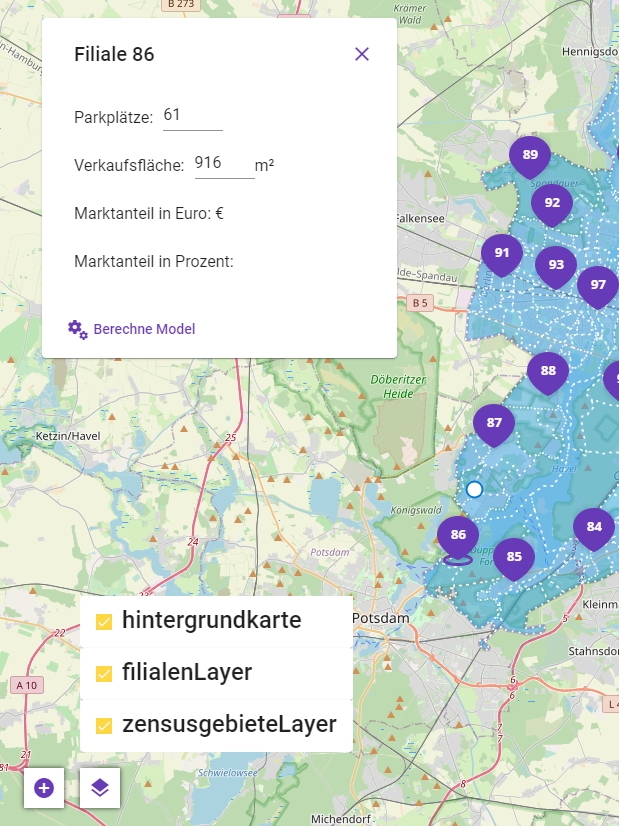
\includegraphics[scale=0.5]{resources/images/toolset.png}}
	\caption{Bildschirmausschnitt der UI-Elemente}
	\label{img:toolset}
\end{figure}

Bei der Umsetzung der UI-Elemente wurde auf die Komponenten-Bibliothek \emph{Angular Material} für fertige UI Komponenten zugegriffen \footcite{team_angular_material}.
Zu den benutzen Komponenten zählen Material Button \footcite{team_angular_material_button}, Icon \footcite{team_angular_material_icon}, Card \footcite{team_angular_material_card}, List \footcite{team_angular_material_list}, Input \footcite{team_angular_material_input} sowie Checkbox \footcite{team_angular_material_checkbox}.

Um eine bessere Visualisierung einzelner Featurelayer zu ermöglichen, sollen die Layer einzeln aus- beziehungsweise eingeblendet werden können.
Dies geschieht im Werkzeug Layermanager.
Hierzu müssen also innerhalb des Werkzeuges alle Layer angezeigt werden und über eine Checkbox die Sichtbarkeit verändert werden können.\\
Für die Konfiguration des Layermanagers werden zunächst über den BaseMap-Service alle Layer der Karte abgerufen.
Aus den Layer-Objekten werden nun Name- und Sichtbarkeit -Eigenschaften in jeweils ein neues LayerManagerEntry-Objekt extrahiert.
Im Layermanager können nun der Name und die Sichtbarkeit pro Layer dargestellt werden, wobei die Sichtbarkeit als Checkbox dargestellt wird.
Mit der Interaktion einer Checkbox wird über den zugehörigen Namen der entsprechende Layer im BaseMap-Service identifiziert und das \emph{Visible} Attribut angepasst.
Der Layermanager erscheint als Fenster nach Aktivierung des entsprechenden Knopfes (Icon: \emph{layer}, siehe Abbildung \ref{img:toolset}).

\begin{lstlisting}[language=JavaScript, caption={Layermanager}]
	
type LayerManagerEntry = { layerIdentifier: LayerIdentifier, visibility: boolean };

public layerManagerEntries: LayerManagerEntry[];

this.layerManagerEntries = baseMapService.getLayers().getArray().map(layer => {
	return {
		layerIdentifier: layer.get('name'),
		visibility: layer.getVisible()
	} as LayerManagerEntry;
});

setLayerVisibility(event: any, layerIdentifier: LayerIdentifier): void {
	if (event.checked) {
		//  show layer
		this.baseMapService.getLayers().getArray().find(layer => layer.get('name') === layerIdentifier).setVisible(true);
	} else {
		//  hide layer
		this.baseMapService.getLayers().getArray().find(layer => layer.get('name') === layerIdentifier).setVisible(false);
	}
}
\end{lstlisting}

Vervollständigt wird das Werkzeug-Set durch die Interaktion eine neue Filiale auf der Karte zu setzen.
OpenLayers bietet hierzu eine Draw-Interaktion, die es erlaubt einer Layersource ein neues Feature hinzuzufügen.

\begin{lstlisting}[language=JavaScript, caption={Draw-Interaktion}]

private addDrawInteraction(): void {
	this.drawInteraction = new Draw({
		type: GeometryType.POINT,
		source: this.tempFilialeLayer.getSource(),
		style: NEW_STORE_INTERACTION_STYLE
	});
	
	this.drawInteraction.on('drawend', (drawEndEvent) => {
		const feature = drawEndEvent.feature;
		
		// new feature needs an new ID or OL Fails with https://openlayers.org/en/v6.3.1/doc/errors/#30
		feature.setId(new Date().getTime());
		featureService.addFiliale(feature);
		this.deactivateAddFiliale();
	});
	this.baseMapService.addInteraction(this.drawInteraction);
}
\end{lstlisting}

In der Initialisierung der Interaktion wird festgelegt, dass nur Punkte erstellt werden können, sowie über einen \emph{NEW\_STORE\_INTERACTION\_STYLE} wird dem Punkt ein eigener Style zugewiesen (ersichtlich in Abbildung \ref{img:toolset}).
Ebenso wird ein temporärer Layer für die neu gesetzte Filiale für die Dauer der Interaktion definiert.
Da auf der neuen Filiale die Attribute Parkplätze und Verkaufsfläche, sowie die Attraktivität noch nicht gesetzt wurden, ist es einfacher für die Interaktionsdauer einen temporären Layer zu verwenden, der nach Interaktionsende das erstellte Feature an den Feature-Service übergibt, wo die fehlenden Attribute gesetzt werden und das Feature in den Filiallayer übertragen wird. 
Sobald die Interaktion der Karte hinzugefügt wurde, muss lediglich bei Aktivierung der temporäre Layer der Karte hinzugefügt werden, damit die Interaktion sichtbar ist.
Ebenso müssen andere Interaktionen, vor Allem die Feature-Selektierung der Filialen und Gebiete (Implementierung erfolgt im späteren Verlauf des Kapitels), deaktiviert werden, damit es hierbei nicht zu ungewollten, parallelen Interaktionsaufrufen kommt.
Sobald eine neue Filiale gesetzt wurde, muss der Layer wieder entfernt, die Interaktion deaktiviert und andere Interaktionen reaktiviert werden.
Aktiviert wird die Interaktion über den entsprechenden Knopf auf der Karte (Icon: \emph{add\_icon}, siehe Abbildung \ref{img:toolset}).

Für die Platzierung im DOM werden beide Werkzeuge in einer Werkzeug-Set Komponente zusammengefasst, die ein einheitliches Styling erlaubt.

Als nächstes muss das Objektfenster, welches bei Selektion eines Features geöffnet werden soll und wichtige Informationen über die Filiale oder das Gebiet enthält, implementiert und in den DOM gesetzt werden.\\
Das Objektfenster ist ein Fenster welches sich wie schon der Layermanager über die Karte legt und Informationen über ein ausgewähltes Feature bietet. 
Selektiert können sowohl Filialen als auch Zensusgebiete werden.
Im Falle einer Filiale soll das Objektfenster auch die Berechnung des Huff-Modells für diese Filiale ermöglichen.\\
Über einen Objektfenster-Service wird das momentan ausgewählte Feature in Form eines \emph{Obervables} \footcite{rxjs_observable} bereitgestellt und ist jederzeit abrufbar.
In Angular erfolgt dieser Aufruf über eine gesetzte \emph{Subscription} \footcite{rxjs_subscription} auf ein Observable.
In einer Angular Anwendung werden Komponenten über mehrere Lifecycle-Zyklen instanziiert, die eine besondere Datenübertragung innerhalb der Anwendung erfordern.
So erfolgt ein initiales Rendering des Templates und der Daten und Änderungen werden über eine \emph{ChangeDetection} erkannt und neu gerendert.
Um Fehler während des ChangeDetection-Lifecycles zu verhindern, erfolgt die Datenübertragung mit Obersvables \footcite{angular_lifecycle}.\\
Im Fall des Objektfensters subscribed die Komponente sich auf das \emph{currentlySelectedFeature\$} des Objektfenster-Services.
Dies bedeutet die Komponente erhält über ein Event direkt die neuesten Änderungen sobald sich das Observable ändert. 
Es erfolgt also kein expliziter, synchroner Datenaufruf, sondern das Observable sendet asynchron Änderungen an alle Subscriber.
Somit kann die Selektierung eines neuen Features problemlos an das Objektfenster weitergeleitet werden und die neuen Daten werden korrekt dargestellt. \\
Das Objektfenster für Filialen zeigt die folgenden Informationen:

\begin{itemize}
	\item Id
	\item Parkplätze
	\item Verkaufsfläche in Quadratmetern
	\item Marktanteil in Euro \footnote{\label{afterCalc}Nach Berechnung des Huff-Modells}
	\item Marktanteil in Prozent \cref{afterCalc}
\end{itemize}

Für ein Gebiet werden folgende Informationen angezeigt:

\begin{itemize}
	\item Id
	\item Einwohner
	\item Kaufkraft in Euro (Durchschnitt pro Monat pro Person)
	\item Ausgaben für Lebensmittel (Durchschnitt pro Monat pro Haushalt) 
	\item Wahrscheinlichkeitsfaktor (für den Besuch einer Filiale) \cref{afterCalc}
	\item Marktanteil der Filiale im Gebiet in Euro \cref{afterCalc}
	\item Marktanteil der Filiale im Gebiet in Prozent \cref{afterCalc}
\end{itemize}

Die Informationen zu Parkplätzen und Verkaufsfläche werden über ein Input-Feld dargestellt (siehe Abbildung \ref{img:filiale}).
Diese Parameter werden für die Attraktivitätsberechnung der Filiale verwendet und müssen für neue Filialen eingegeben werden.
Bei bestehenden Filialen lässt sich somit aber auch die Berechnung des Huff-Modells für die gleiche Filiale mit verschiedenen Parametern ermöglichen.

\begin{figure}[H]
	\makebox[\textwidth][c]{
		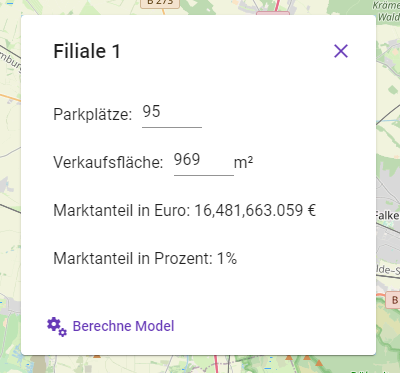
\includegraphics[scale=0.5]{resources/images/filiale_of.png}}
	\caption{Bildschirmausschnitt des Objektfensters einer Filiale}
	\label{img:filiale}
\end{figure}

Das Objektfenster öffnet sich automatisch nach dem Anlegen einer neuen Filiale.
Hierbei werden die Parkplätze und Verkaufsfläche zunächst mit jeweils dem Wert Null angelegt und angezeigt.
Bevor das Huff-Modell berechnet werden kann, müssen valide Werte in beide Felder eingetragen werden, da solange der Knopf deaktiviert ist.
Die Aktivierung des Knopfes erfolgt über die einfache Validierung der Werte auf eine positive Zahl.\\
Der Knopf zur Berechnung des Huff-Modells ruft eine Funktion im Feature-Service auf, die die Berechnung für die ausgewählte Filiale durchführen soll.
Über den Schließ-Knopf (Icon: \emph{close}, siehe Abbildung \ref{img:filiale}) wird das Objektfenster geschlossen und der Wert des Observables \emph{currentlySelectedFeature\$} auf \emph{null} gesetzt.

Mit der Implementierung des Objektfensters sind nun sämtliche Komponenten der Anwendung bereit, die für Berechnung des Huff-Modells und anschließenden farbliche Einfärbung der Zensusgebiete erforderlich sind.

Die Berechnung des Huff-Modells erfolgt im Feature Service.
Die für das Huff-Modell erforderliche Parameter Attraktivität A und Faktor der Attraktivität $\alpha$, sowie Distanz D und Faktor der Distanzfunktion $\beta$ müssen bestimmt werden.
Wie bereits im Kapitel \ref{subsec:gravitationmodel} zum Gravitationsmodell nach Huff erläutert, sind die Faktoren $\alpha$ und $\beta$ für die Berechnung im realen Wirtschaftsumfeld empirisch anhand von realen Markt- und Wirtschaftsdaten aus Umfragen mit Kunden zu analysieren und zu bestimmen.
Für den Prototypen sind diese Werte auf 1,5 für $\alpha$ und 1,5 für $\beta$ festgelegt.
Angenommen wird also, dass je attraktiver eine Filiale ist desto Wahrscheinlicher auch ein Besuch eines Kunden ist.
Ebenso, je näher ein Kunde an einer Filiale wohnt desto wahrscheinlicher ist auch hier der Besuch der Filiale.\\
Die Attraktivität A der Filiale wird über die Summe der Parkplätze und Verkaufsfläche berechnet.
Je größer eine Filiale desto größer ist wahrscheinlich das Sortiment und die Menge der Lebensmittel.
Und je mehr Parkplätze vor der Filiale vorhanden sind desto mehr Kunden können angezogen werden, die einen weiteren Anreiseweg haben oder mehr auf einmal einkaufen wollen.
Für die Berechnung der Attraktivität sind viele weitere Parameter denkbar jedoch bieten die Anzahl der Parkplätze und die Verkaufsfläche in Quadratmetern aus den aufgeführten Gründen eine fundierte Grundlage für die Bewertung der Attraktivität.\\
Die Distanz D der Filiale zu den Gebieten ist eine einfache Distanzberechnung in OpenLayers vom Standort der Filiale zum Mittelpunkt des jeweiligen Gebiets.
Zunächst werden aus den Features der Gebiete über \emph{Type Assertion} Multipolygone über die OpenLayers interne Funktionen zur Mittelpunktbestimmung bieten.
Da Multipolygone mehrere Mittelpunkte haben, wird der erste Eintrag aus dem Array gewählt.\\
OpenLayers bietet für die Längen- und Größenberechnung verschiedene Funktionen, die sich in der Berechnung unter Einbezug der Projektion unterscheiden \footcite{openlayers_measure_example}.
Die Koordinaten der Filiale und des Mittelpunkts des Gebiets werden zu einem \emph{LineString} Objekt zusammengefasst \footcite{openlayers_linestring}.
Von dieser Linie wird nun die Länge berechnet.
Wird die einfache Berechnung \emph{LineString.getLength()} verwendet, berechnet OpenLayers die Länge anhand von Orthodromen \footcite{orthodrome_frassek} oder der Großkreisdistanz \footcite{great_circle_distance}.
Wenn auch hervorragend für Flugdistanzen verwendbar, lässt diese Berechnung die Ergebnisse für Entfernungen auf dem Boden ungenau werden.\\
Über das \emph{Sphere} Paket von OpenLayers lässt sich aber eine Länge anhand der Projektion der Karte berechnen, welches zu den gewünschten Ergebnissen führt \footcite{openlayers_sphere}.

\begin{lstlisting}[language=JavaScript, caption={Huff-Modell Variablen und Parameter}]
	
	// distance decay
	const DIST_DECAY = 1.5;
	// attractiveness enhancement factor
	const ATT_ENHANCE_FACTOR = 1.5;
	
	const centerCoordinates = (gebietFeature.getGeometry() as MultiPolygon).getInteriorPoints().getFirstCoordinate();
	
	const distance = ol_sphere.getLength(new LineString([filialCoordinates, centerCoordinates]), {projection: 'EPSG:3857'});
	
	const attractiveness = filiale.parkingSpaces + filiale.salesArea;
	
\end{lstlisting}

Über den Knopf \emph{Berechne Huff-Modell} (Icon: \emph{miscellaneous\_services}, siehe Abbildung \ref{img:filiale}) im Objektfenster der ausgewählten Filiale wird die Id der Filiale an den Feature Service übergeben und die Berechnung gestartet.
Über die Id wird das Feature der entsprechenden Filiale im Filiallayer identifiziert und kann bearbeitet werden.\\
Die Wahrscheinlichkeit des Besuchs eines Gebiets für die ausgewählte Filiale innerhalb des gesamten Filialnetzes ergibt sich, wenn die Wahrscheinlichkeit der ausgewählten Filiale ins Verhältnis zur Netzwahrscheinlichkeit gesetzt wird.
Für die Filiale errechnet sich die Wahrscheinlichkeit des Besuchs der einzelnen Gebiete daher anhand von zwei \emph{ForEach} Schleifen.
Zunächst wird über alle Gebiete iteriert, um die Wahrscheinlichkeit sämtlicher Gebiete für die ausgewählte Filiale zu berechnen.
In der Schleife der Gebiete muss für jedes Gebiet über die Filialen iteriert werden, um die Menge der Wahrscheinlichkeiten aller Filialen zu dem Gebiet zu berechnen.

\begin{lstlisting}[language=JavaScript, caption={Berechnung des Huff-Modells}]
	
	zensusgebiete.forEach(gebiet => {
		// probability for all stores
		let netProbability = 0;
		
		// probability for the selected store alone
		const storeProbability = Math.pow(filiale.attractiveness, this.ATT_ENHANCE_FACTOR) / Math.pow(distance, this.DIST_DECAY);
		
		filialen.forEach(store => {
			netProbability += Math.pow(store.attractiveness, this.ATT_ENHANCE_FACTOR) / Math.pow(this.calculateDistancesForFiliale(store.coordinates, gebiet.coordinates), this.DIST_DECAY);
		});
	
		// probability inside net of stores
		gebiet.probability = storeProbability / netProbability;

		// marketshare
		gebiet.marketShare = gebiet.spendituteGroc * gebiet.probability;
		gebiet.marketSharePercentage = gebiet.marketShare / gebiet.spendituteGroc;
	});
\end{lstlisting}

Nachdem jedes Gebiet Besuchswahrscheinlichkeiten ausgerechnet bekommen hat, wird der Marktanteil prozentual sowie monetär für ein besseres Verständnis sowie eine bessere Einordnung errechnet.
Hierzu werden die Ausgaben des Gebiets für Lebensmittel im Monat mit der Wahrscheinlichkeit des Besuchs multipliziert, um den Anteil der Lebensmittelausgaben in Euro des Gebiets für die ausgewählte Filiale zu errechnen.
Wird dieser Betrag nun ins Verhältnis zu den Gesamtausgaben für Lebensmittel im Gebiet gesetzt, errechnet sich der prozentuale Anteil.
Erfolgten diese Schritte für alle Gebiete und werden die Beträge des Anteils der Ausgaben der Filiale und der Gesamtausgaben pro Gebiet summiert, ergibt sich der Marktanteil der Filiale im Netz in Euro und, im Verhältnis zu einander, in Prozent.

\begin{lstlisting}[language=JavaScript, caption={Martkanteil Berechnung}]
	
	let marketShareTotal = 0;
	let totalMarketExpenditure = 0;
	this._zensusMap.forEach((gebiet: ZensusProperties) => {
		marketShareTotal += gebiet.marketShare;
		totalMarketExpenditure += gebiet.spendituteGroc;
	});
	filiale.marketShare = marketShareTotal;
	filiale.marketSharePercentage = marketShareTotal / totalMarketExpenditure;
	
\end{lstlisting}

Bei jeder Berechnung der Wahrscheinlichkeit des Besuchs der Gebiete für die ausgewählte Filiale wird final nun noch das Gebiet eingefärbt.
Hierzu wird auf jedem Feature abhängig der errechneten Wahrscheinlichkeit ein Indikator gesetzt, der einer bestimmten Farbe entspricht.

\begin{lstlisting}[language=JavaScript, caption={Setzen des Einfärbeindikators}]
	
	const probabilityInPercent = gebiet.probability * 100;
	
	if (probabilityInPercent > 80) {
		gebiet.indicator = 1;
	}
	else if (probabilityInPercent < 80 && probabilityInPercent > 70) {
		gebiet.indicator = 2;
	}

	...
	
	else {
		gebiet.indicator = 9;
	}
\end{lstlisting}


Dieser Indikator wird im Renderzyklus der Gebiete innerhalb der \emph{StyleFunction} pro Gebiet ausgelesen und das Gebiet entsprechend eingefärbt (ähnlich zur StyleFunction der Filialen \ref{code:filialStyle}).

\begin{lstlisting}[language=JavaScript, caption={Einfärben der Gebiete}]
	
	protected readonly colorGradient: ColorInterface[] = [
		{ gravitationalRing: 1, value: 'rgb(255, 0, 0)'},
		{ gravitationalRing: 2, value: 'rgb(255, 70, 0)'},
		{ gravitationalRing: 3, value: 'rgb(255, 105, 0)'},
		{ gravitationalRing: 4, value: 'rgb(255, 134, 0)'},
		{ gravitationalRing: 5, value: 'rgb(255, 160, 0)'},
		{ gravitationalRing: 6, value: 'rgb(246, 185, 0)'},
		{ gravitationalRing: 7, value: 'rgb(241, 206, 31)'},
		{ gravitationalRing: 8, value: 'rgb(236, 227, 66)'},
		{ gravitationalRing: 9, value: 'rgb(231, 247, 98)'}
	];
	
	const gebieteStyle = new Style({
		stroke: new Stroke({
			color: 'white',
			width: 2,
			lineDash: [0.1, 7]
		}),
		fill: new Fill({
			color: 'rgba(52, 164, 235, 0.5)'
		})
	});

	const gebieteStyleFunction = (feature, resolution) => {
		const indicator = feature.indicator;
		
		if (!indicator) {
			return this.ezbLineStyle;
		}
		const color = colorGradient.find(color => color.gravitationalRing === indicator).value;
		gebieteStyle.getFill().setColor(color);
		return gebieteStyle;
	}
\end{lstlisting}

Für die Farben der einzelnen Gravitationsringe wurde ein Farbgradient von Rot zu Gelb gewählt.
Besonders hohe Besuchswahrscheinlichkeiten werden mit einer Farbe aus dem roten Spektrum des Gradienten dargestellt und mit abnehmender Wahrscheinlichkeit wird das Gebiet zunehmend gelber.
Das berechnete Modell kann in der Abbildung \ref{img:calc_modell} begutachtet werden.

\begin{figure}[H]
	\makebox[\textwidth][c]{
		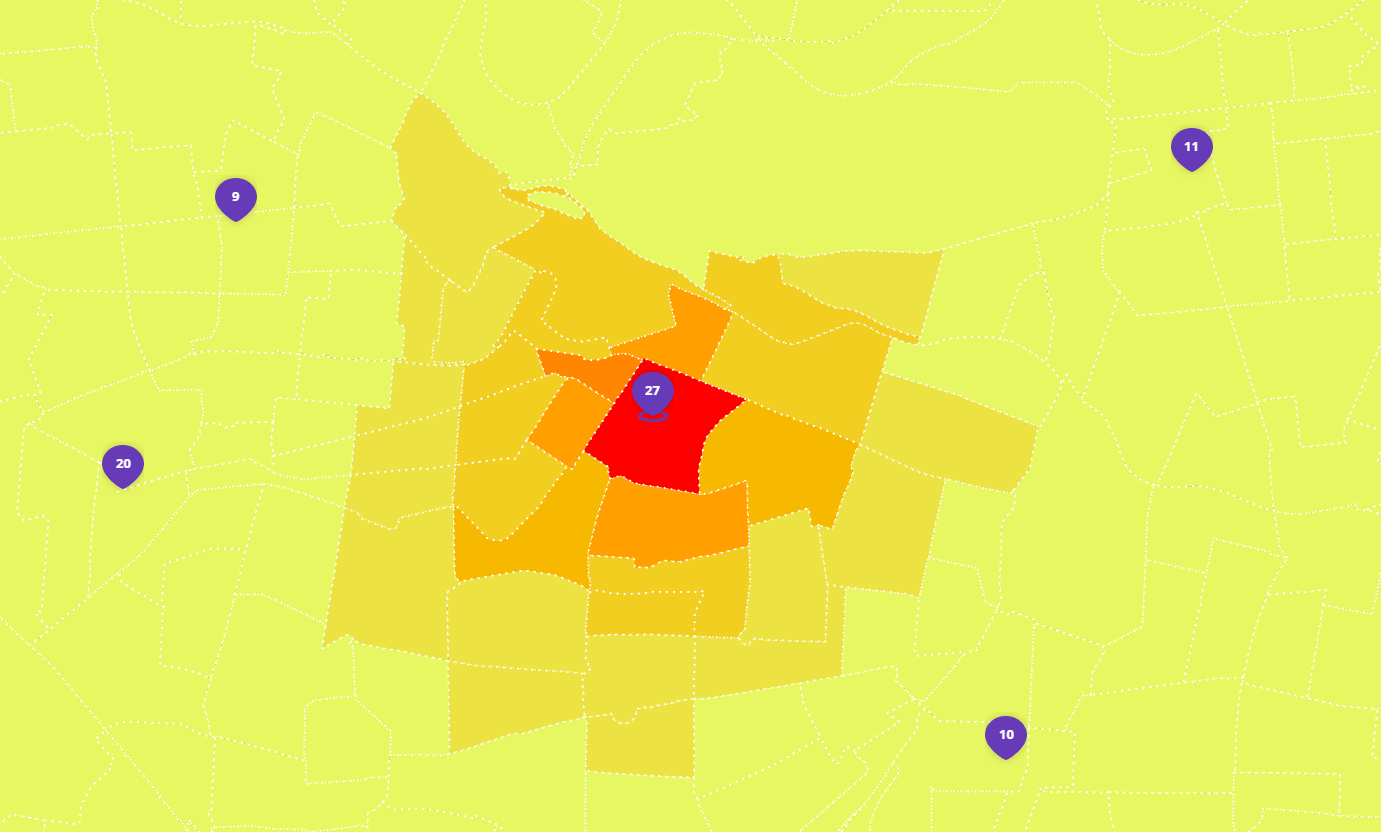
\includegraphics[scale=0.4]{resources/images/modell_calculated.png}}
	\caption{Bildschirmausschnitt des Prototypen nach der Berechnung des Huff-Modells für Filiale 27}
	\label{img:calc_modell}
\end{figure}
 \clearpage
\chapter{Auswertung}
\section{Performance}
\section{Fazit/ Ausblick} \clearpage
%\chapter{Beispiele} \label{c:beispiele}

Im Kapitel Beispiele (siehe \autoref{c:beispiele}) werden die möglichen Funktionen und\index{und} Möglichkeiten dies LaTeX-Dokuments demonstriert.

\section{Quelltext}

Nachfolgend der \autoref{lst:helloworld}.

\begin{lstlisting}[caption={Hello World}, captionpos=b, label={lst:helloworld}]
/**
* The HelloWorldApp class implements an application that
* simply prints "Hello World!" to standard output.
*/
class HelloWorldApp {
	public static void main(String[] args) {
		System.out.println("Hello World!"); // Display the string.
	}
}
\end{lstlisting}

\section{Bild}

\begin{wrapfigure}{R}{0.5\textwidth}
	\centering
	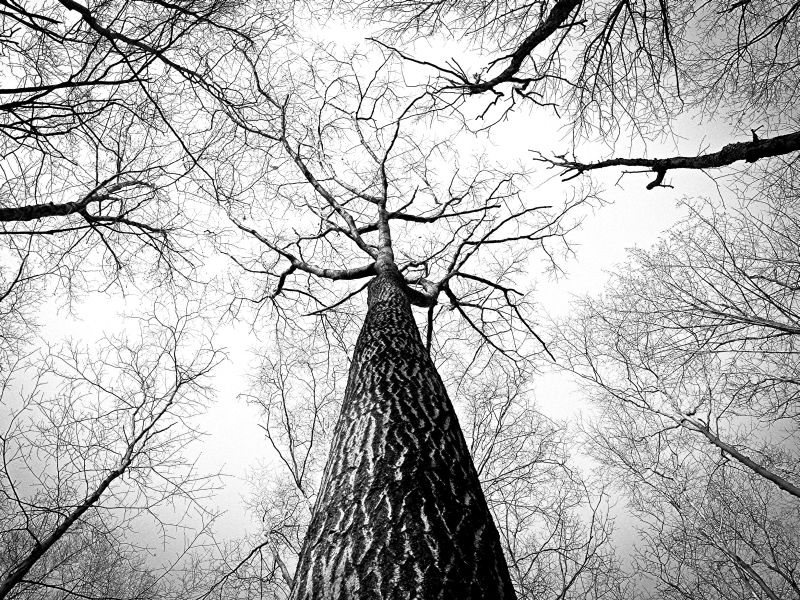
\includegraphics[width=0.5\textwidth]{resources/images/example}
	\caption{Beispielbild {\cite{PEXELS2015}}}
\end{wrapfigure}

Die rechts zu sehende Grafik demonstriert die Möglichkeiten des Paketes \glqq wrapfig\grqq . Grafiken innerhalb einer \glqq wrapfigure\grqq{} können entweder links oder rechts von Text umlaufen werden.

Die nachfolgende \autoref{img:beispielbild} demonstriert die Darstellung\index{Darstellung} eines \glqq *.jpg\grqq{} Bildes innerhalb des Textes (beim Einfügen kann auf die Endung verzichtet werden, solange der Name einzigartig ist). Zusätzlich enthält dieses einen Untertitel der über das bereits verwendete Label verlinkt werden kann. Der Untertitel\index{Untertitel} erscheint im \gls{abbvz}.

\section{Text Formatierungen und sonstiges}
Dieser Text enthält eine Fußnote\footnote{Fußnoten sind Anmerkungen, die im Druck-Layout aus dem Fließtext ausgelagert werden, um den Text flüssig lesbar zu gestalten.}.

\subsection{Listen}
Listen könne sowohl mit Bullet points als auch mit Zahlen erstellt werden
\begin{itemize}
	\item Eine Liste mit Bullet points
	\item Ein weiteres Element
\end{itemize}

\begin{enumerate}
	\item Eine Liste mit Zahlen
	\item Ein weiteres Element
\end{enumerate}

\subsection{Text Hervorhebungen}
\begin{quote}
	The problem with internet quotes is that you can't always depend on their accuracy \par\raggedleft--- \textup{Abraham Lincoln, 1864}
\end{quote}

\epigraph{problem}{Ab Lincoln}
\epigraph{The problem with internet quotes is that you can't always depend on their accuracy}{Abraham Lincoln, 1864}

\begin{figure}[H]
	\centering
	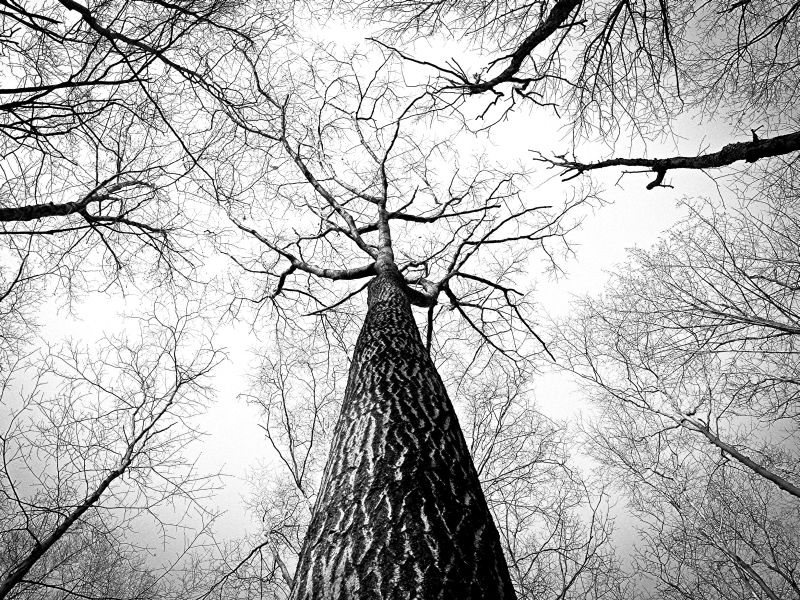
\includegraphics[width=0.7\textwidth]{resources/images/example}
	\caption{Beispielbild {\cite{PEXELS2015}}}
	\label{img:beispielbild}
\end{figure}

\section{Tabelle}

Nachfolgend \autoref{tbl:DigitalesZertifikat}.

\begin{table}[H]
	\begin{center}
		\renewcommand{\arraystretch}{1.3}
		\begin{tabular}{|l|}
			\hline
			\textbf{Inhaber:}\\
			Alice \\ \hline
			\textbf{Peer (Ersteller):}\\
			Bob \\ \hline
			\textbf{Öffentlicher Schlüssel des Inhabers:}\\
			F2 D2 0E ED FA 4E 9E 0A F2 DD 23 8A 32 44 F3 E9 \\ \hline
			\textbf{Gültigkeit:}\\
			2015-07-01 – 2016-06-30 \\ \hline
		\end{tabular}
	\end{center}
	\caption{Digitales Zertifikat}
	\label{tbl:DigitalesZertifikat}
\end{table}

\section{Long-Table}

Die \glqq Long-Table\grqq kann über definierte Header und Footer über Seitenumbrüche hinweg angezeigt werden.

\begin{longtable}{|l|l|l|l|}
	\hline
	\multicolumn{1}{|c}{\textbf{Version}} & \multicolumn{1}{|c}{\textbf{Codename}} &
	\multicolumn{1}{|c}{\textbf{API}} &
	\multicolumn{1}{|c|}{\textbf{Verteilung}} \\ \hline
	\endfirsthead
	
	\multicolumn{4}{c}{Fortsetzung - Verteilung der Androidversionen (Stand 01.02.2016)}\\ \hline
	\multicolumn{1}{|c}{\textbf{Version}} & \multicolumn{1}{|c}{\textbf{Codename}} &
	\multicolumn{1}{|c}{\textbf{API}} &
	\multicolumn{1}{|c|}{\textbf{Verteilung}} \\ \hline 
	\endhead
	
	\multicolumn{4}{c}{Fortsetzung auf nachfolgender Seite}
	\endfoot
	
	\caption{Verteilung der Androidversionen (Stand: 01.02.2016)}
	\label{tab:androidverteilung}
	\endlastfoot
	
	2.2 & Froyo & 8 & 0.1\%\\ \hline
	2.3.3 - 2.3.7 & Gingerbread & 10 & 2.7\%\\ \hline
	4.0.3 - 4.0.4 & Ice Cream Sandwich & 15 & 2.5\%\\ \hline
	4.1.x & Jelly Bean & 16 & 8.8\%\\ \cline{1-1} \cline{3-4}
	4.2.x &  & 17 & 11.7\%\\ \cline{1-1} \cline{3-4}
	4.3 &  & 18 & 3.4\%\\ \hline
	4.4 & KitKat & 19 & 35.5\%\\ \hline
	5.0 & Lollipop & 21 & 17.0\%\\ \cline{1-1} \cline{3-4}
	5.1 &  & 22 & 17.1\%\\ \hline
	6.0 & Marshmallow & 23 & 1.2\%\\ \hline
\end{longtable}

\section{Literaturverweis}

Weil für die alte\index{alte} und die neue Rechtschreibung verschiedene Trennregeln\index{Trennregeln} gelten, sind Deutsch mit alter Rechtschreibung und Deutsch mit neuer Rechtschreibung zwei verschiedene Sprachen (\cite{Knappen2009}, S. 192).

\section{Onlineverweise}

Siehe Google.de \cite{Google2015}.

\section{Glossar}
Der Glossar enthält die Beschreibung verwendeter Begriffe für das bessere Verständnis gegenüber dem Leser. Beispiele sind: \gls{berlin}, \gls{outsourcing}, \gls{asp}, \gls{policy} und \gls{pcie}.

\section{Abkürzungsverzeichnis}
Das Abkürzungsverzeichnis listet alle verwendeten Abkürzungen auf. Einige Beispiele sind \gls{leh}. Die erneute Verwendung zeigt nur noch die Abkürzung: \gls{leh}. \clearpage

%Anhang
\pagenumbering{Alph}

%Abbildungsverzeichnis
\listoffigures \clearpage
%Tabellenverzeichnis
\listoftables \clearpage
%Quelltextverzeichnis
\lstlistoflistings \clearpage
%Stichwortverzeichnis
\printindex \clearpage
%Glossar
\printglossary[title={Glossar}] \clearpage
%Abkürzungsverzeichnis
\printglossary[style=dottedlocations,type=\acronymtype,title={Abkürzungsverzeichnis}] \clearpage

%Literaturverzeichnisse (getrennt nach Stichwort)
\printbibliography[title={Literaturverzeichnis}]\clearpage
\printbibliography[heading=bibintoc, keyword={online}, title={Onlinequellen}]\clearpage
\printbibliography[heading=bibintoc, keyword={image}, title={Bildquellen}]\clearpage

% Anhang
\appendix

\chapter{}
\addcontentsline{toc}{chapter}{Anhang A}

\section{Diagramm}

\section{Tabelle}

\section{Screenshot}

\section{Graph}

\end{document}